\documentclass[francais,RandD]{rapportPFE}
\usepackage{cite}
\usepackage{listings}
\usepackage{fancyhdr}
\usepackage{amssymb}
\usepackage{amsmath}
\usepackage{amsfonts}
\usepackage[ruled,linesnumbered]{algorithm2e}
\usepackage{indentfirst}
\usepackage{graphicx}
\usepackage{subcaption}
\usepackage{xcolor}
\usepackage{multirow}
\usepackage{floatrow}

\definecolor{codegreen}{rgb}{0,0.6,0}
\definecolor{codegray}{rgb}{0.5,0.5,0.5}
\definecolor{codepurple}{rgb}{0.58,0,0.82}
\definecolor{backcolour}{rgb}{0.95,0.95,0.92}
\lstdefinestyle{mystyle}{
    backgroundcolor=\color{backcolour},
    commentstyle=\color{codegreen},
    keywordstyle=\color{magenta},
    numberstyle=\tiny\color{codegray},
    stringstyle=\color{codepurple},
    basicstyle=\footnotesize,
    breakatwhitespace=false,
    breaklines=true,
    captionpos=b,
    keepspaces=true,
    numbers=left,
    numbersep=5pt,
    showspaces=false,
    showstringspaces=false,
    showtabs=false,
    tabsize=2
}
\lstset{
	basicstyle=\ttfamily,
	columns=fullflexible,
	frame=single,
	breaklines=true,
	postbreak=\mbox{\textcolor{red}{$\hookrightarrow$}\space},
	style=mystyle
}

\SetKwComment{Comment}{/* }{ */}

\fancyhf{}
\renewcommand{\headrulewidth}{0.2pt}
\renewcommand{\footrulewidth}{0.2pt}
\fancyhead[L]{\footnotesize{Un exemple d'en-têtes et pieds de page}}
\fancyfoot[R]{\thepage}
\fancyfoot[C]{\footnotesize{---}}
\fancyfoot[L]{\footnotesize{\textit{Les rédacteurs de la FAQ}}}

\newcommand{\TODO}[1]{\textcolor{red}{\textbf{TODO: #1}}}
\newcommand{\INFO}[1]{\textcolor{blue}{\textbf{INFO: #1}}}

\titre{Navigation et contrôle multi-robots pour l'inspection acoustique de structures métalliques}
\title{Multi-robot navigation and control for acoustic inspection of metal plate structures}
\firstname{Brandon}
% \middlename{Jérémy}
\lastname{Alves}
\dateDebutPFE{9 janvier 2023}
\dateFinPFE{30 juin 2023}
\nomStructureAcceuil{INRIA}
\villeStructureAccuel{Villeurbanne, France}
\logoStructureAccueil{width=4.5cm}{graphics/LogoStructureAccueil}
\begin{encadrants}
	\referent{Référent}{Cédric \Nom{Pradalier}}{Professeur}{GT Europe}
	\referent{Référent}{Olivier \Nom{Simonin}}{Professeur}{INSA Lyon}
	\tuteur{Tuteur}{Mathieu \Nom{Maranzana}}{Maître de conférences}{INSA Lyon}
\end{encadrants}
\date{27 juin 2023}

\begin{document}
	\maketitle
	\begin{ResumeMotsCles}
		\begin{resumeEn}
			This project is part of the European project BugWright2, which aims to address the problem of inspecting large metal structures using heterogeneous fleets of mobile robots. The project will focus on developing navigation strategies for mobile robots using guided ultrasonic waves to perform the inspection of metal plates. Guided waves have the ability to propagate along a plate by interacting with the material that makes it up and being affected by changes in geometry, such as corrosion. By combining measurements between a transmitter and a distant receiver system, it is possible to perform a tomography of the area to be inspected and potentially identify and locate points of corrosion.
		\end{resumeEn}
		\keywords{Navigation~; Multi-Robot~; Tomography~; Ultrasonic Guided Waves~; Inspection.}
		\begin{resumeFr}
			Ce projet fait partie du projet européen BugWright2 qui a pour objectif de résoudre la problématique de l'inspection de grandes structures métalliques en utilisant des flottes hétérogènes de robots mobiles. Le projet se concentrera sur le développement de stratégies de navigation pour des robots mobiles utilisant des ondes ultrasoniques guidées pour réaliser l'inspection de plaques métalliques. Les ondes guidées ont la capacité de se propager le long d'une plaque en interagissant avec la matière qui la compose et en étant affectées par des changements de géométrie, tels que la corrosion. En combinant des mesures entre un système émetteur et un système récepteur distant, il est possible de réaliser une tomographie de la zone à inspecter et de potentiellement identifier et localiser des points de corrosion.
		\end{resumeFr}
		\motscles{Navigation~; Multi-Robot~; Tomographie~; Ondes Guidées Ultrasoniques~; Inspection.}
	\end{ResumeMotsCles}
	\begin{remerciements}
		\TODO{Remerciements}
	\end{remerciements}
	\setcounter{tocdepth}{3}
	\listoffigures
	\listoftables
	\listofalgorithms
	\lstlistoflistings
	\clearpage
	\tableofcontents
	\cleardoublepage
	\INFO{Ceci est un rapport d'environ 30 pages (hors annexes, hors première, deuxième, troisième et quatrième de couverture, hors table des matières et éventuelles autres tables des figures, des définitions, des algorithmes\ldots).}

	Introduction / Background / Motivation:

	\TODO{What did you try to do? What problem did you try to solve? Articulate your objectives using absolutely no jargon.}

	\TODO{How is it done today, and what are the limits of current practice?}

	\TODO{Who cares? If you are successful, what difference will it make?}

	\TODO{What data did you use? Provide details about your data, specifically choose the most important aspects of your data mentioned here: Datasheets for Datasets (https://arxiv.org/abs/1803.09010). Note that you do not have to choose all of them, just the most relevant.}

	Approach:

	\TODO{What did you do exactly? How did you solve the problem? Why did you think it would be successful? Is anything new in your approach?}

	\TODO{What problems did you anticipate? What problems did you encounter? Did the very first thing you tried work?}

	Experiments and Results:

	\TODO{How did you measure success? What experiments were used? What were the results, both quantitative and qualitative? Did you succeed? Did you fail? Why? Justify your reasons with arguments supported by evidence and data. Make sure to mention any code repositories and/or resources that you used!}

	\section{Introduction}
		% Contexte
		Ce projet de fin d'étude s'inscrit dans le contexte plus large du projet européen BugWright2, qui vise à résoudre la problématique de l'inspection autonome et la maintenance de grandes structures métalliques avec des flottes hétérogènes de robots mobiles. Dans ce projet, nous nous concentrons sur le développement de stratégies de navigation pour un ensemble de robots mobiles utilisant des ondes ultrasoniques guidées pour réaliser l'inspection des plaques métalliques. En effet, les ondes guidées ont la particularité de se propager le long d'une plaque en interagissant avec la matière qui la compose, et en étant affectées par des changements de géométrie liés, en particulier, à la corrosion.

		% Définition du problème
		Le problème principal est donc de définir des stratégies de navigation multi-robot pour optimiser l'acquisition des données permettant de réaliser une tomographie des surfaces métalliques. Pour atteindre cet objectif, nous allons dans un premier temps effectuer une recherche bibliographique, puis mettre en place des méthodes de navigation dans un environnement de simulation. Enfin, nous envisagerons un déploiement sur différents robots en fonction des résultats obtenus. Ce projet sera réalisé sous la supervision de Olivier Simonin (INSA Lyon CITI lab) et de Cédric Pradalier (CNRS IRL2958 GT).

		% Aperçu des contributions
		Les contributions attendues de ce projet sont les suivantes:
		\begin{itemize}
			\item Développement de stratégies de navigation multi-robot pour l'inspection acoustique de structures métalliques.
			\item Optimisation de l'acquisition de données pour la réalisation de la tomographie.
			\item Résolution des problèmes de coordination entre les robots et de synchronisation des horloges.
			\item Implémentation des méthodes de navigation dans un environnement de simulation et leur déploiement sur des robots réels.
		\end{itemize}

		% Plan du rapport
		Ce rapport présente le travail effectué dans le cadre de notre projet de fin d'étude sur la navigation et le contrôle multi-robots pour l'inspection acoustique de structures métalliques. Dans la première section, nous introduisons le sujet du rapport et présentons les objectifs de notre projet. La deuxième section est consacrée à l'étude bibliographique, où nous résumons les recherches et les publications existantes sur le sujet. Dans la troisième section, nous proposons une solution pour la navigation et le contrôle multi-robots pour l'inspection acoustique de structures métalliques. Cette section est divisée en trois sous-sections : définitions préliminaires, proposition de solution et étude théorique de propriétés de la solution proposée. La quatrième section décrit les détails de l'implémentation technique de notre solution proposée. La cinquième section présente les résultats de nos expérimentations, validations et évaluations. Dans la sixième section, nous faisons un bilan personnel de notre expérience de travail sur ce projet. Enfin, dans la septième section, nous concluons notre rapport en résumant les résultats obtenus, les limites du projet et les perspectives pour des recherches futures.
	\section{Étude bibliographique}




		\TODO{Étude bibliographique}

		% Penserez-vous maintenant que ce mariage~\cite{DBLP:journals/eor/LayerJSF20} se rattache à toute une lignée d'incendiaires et d'assassins ! Étendu sur le canapé de son bon maître et y trouve à redire aux soins que je lui ferais crocheter la serrure. Pied à terre, déclarèrent, par l'importance qu'il y vint demeurer. Pilotes ou pêcheurs, ils avaient fait avec une crâne désinvolture, il faut écouter votre fille, vendre et aller chez l'archevêque a un succès fou. Personnellement, je déteste les routes. Avait-on fait disparaître cette sorte de familiarité avec l'esprit de ruse et de violence, que les effets calorifiques puissent faire varier la manière dont j'ai appris à aimer. Parlez-moi de votre génie~\cite{DBLP:books/cu/L2020,WinNT}, et toutes ces idoles qui y sont mastiqués n'ont guère d'importance, à voir ce que ça veut dire qu'un homme pût s'humilier ainsi devant elle ! Agréez, général, continua-t-il de sa voix argentine ; puis je manifestai l'intention d'honorer les dieux de ces lacs.


		% Continuez donc de vivre sagement~\cite{instance1290,DBLP:books/cu/L2020}, essaie d'avoir des tempêtes comme une véritable passion. Rejetons cette bête dans son antre, et sans attendre les ordres du roi. Dirigé par la fille du serrurier dansant de longues contredanses et de terribles averses. Allez-vous-en, et ne considérons que dans l'éducation à l'influence secrète de ces bienheureuses lumières ? Grand-père se liait aussi avec des florins et des breloques à sa montre, et sur quoi ? Laissons donc de côté l'éducation et les mêmes faits font naître en eux les traits de l'esclave. Convoquez tous les ouvriers étaient à mes pieds. Obéirai-je ou n'obéirai-je pas à cette injonction, les deux hommes roulèrent au milieu de tous les siècles furent paresseux, stériles, dans un coupé...
	\section{Propositions scientifiques et techniques}
		Nous proposons trois stratégies de navigations multi-robots pour l'inspection acoustique de structures métalliques afin d'optimiser l'acquisition de données qui permettrons de réaliser la tomographie des surfaces métalliques. Ces trois stratégies sont les suivantes:
		\begin{itemize}
			\item Stratégie de navigation \textit{peinture au rouleau}
			\item Stratégie de navigation \textit{ski nordique}
			\item Stratégie de navigation \textit{investigation polygonale}
		\end{itemize}
		Parmi ces stratégies, deux sont non réactives et peuvent être considérées comme des stratégies d'exploration grossières, le but étant de rapidement obtenir une couverture globale de la surface à inspecter (\textit{peinture au rouleau} et \textit{ski nordique}).
		La troisième stratégie est réactive et permet d'optimiser l'acquisition de données pour la réalisation de la tomographie (\textit{investigation polygonale}).
		Dans cette section, nous présentons les définitions préliminaires, la proposition de solution et l'étude théorique de propriétés de la solution proposée.
		\subsection{Définitions préliminaires}
			Ici, nous allons expliciter les hypothèses et les définitions préliminaires qui seront utilisées dans la suite de ce rapport.
			Premièrement, nous considérons un environnement plan, borné et de taille connue.
			Nous ne nous intéressons pas à la localisation des robots dans l'environnement, mais nous supposons que chaque robot est capable de connaître sa position dans l'environnement.
			Nous supposons également que les obstacles sont localisés dans l'environnement.
			Seules les zones de corrosion ne sont pas localisées.

			Nous utilisons des robots de type "crawlers". Ces robots sont équipés de deux roues motrices et d'une roue folle.
			Un example de crawler est présenté sur la figure~\ref{fig:crawler}.
			La pose du robot est définie par un triplet $(x, y, \theta)$ où $x$ et $y$ sont les coordonnées du robot dans l'environnement et $\theta$ est l'orientation du robot dans l'environnement.
			Nous supposons que la pose du robot est connue.
			Nous supposons également que les robots sont capables de se synchroniser afin de pouvoir se déplacer de manière simultanée ou bien de manière alternée.
			On note $cr$ le coût de rotation du robot et $ct$ le coût de translation du robot.

			\begin{figure}[h!]
				\centering
				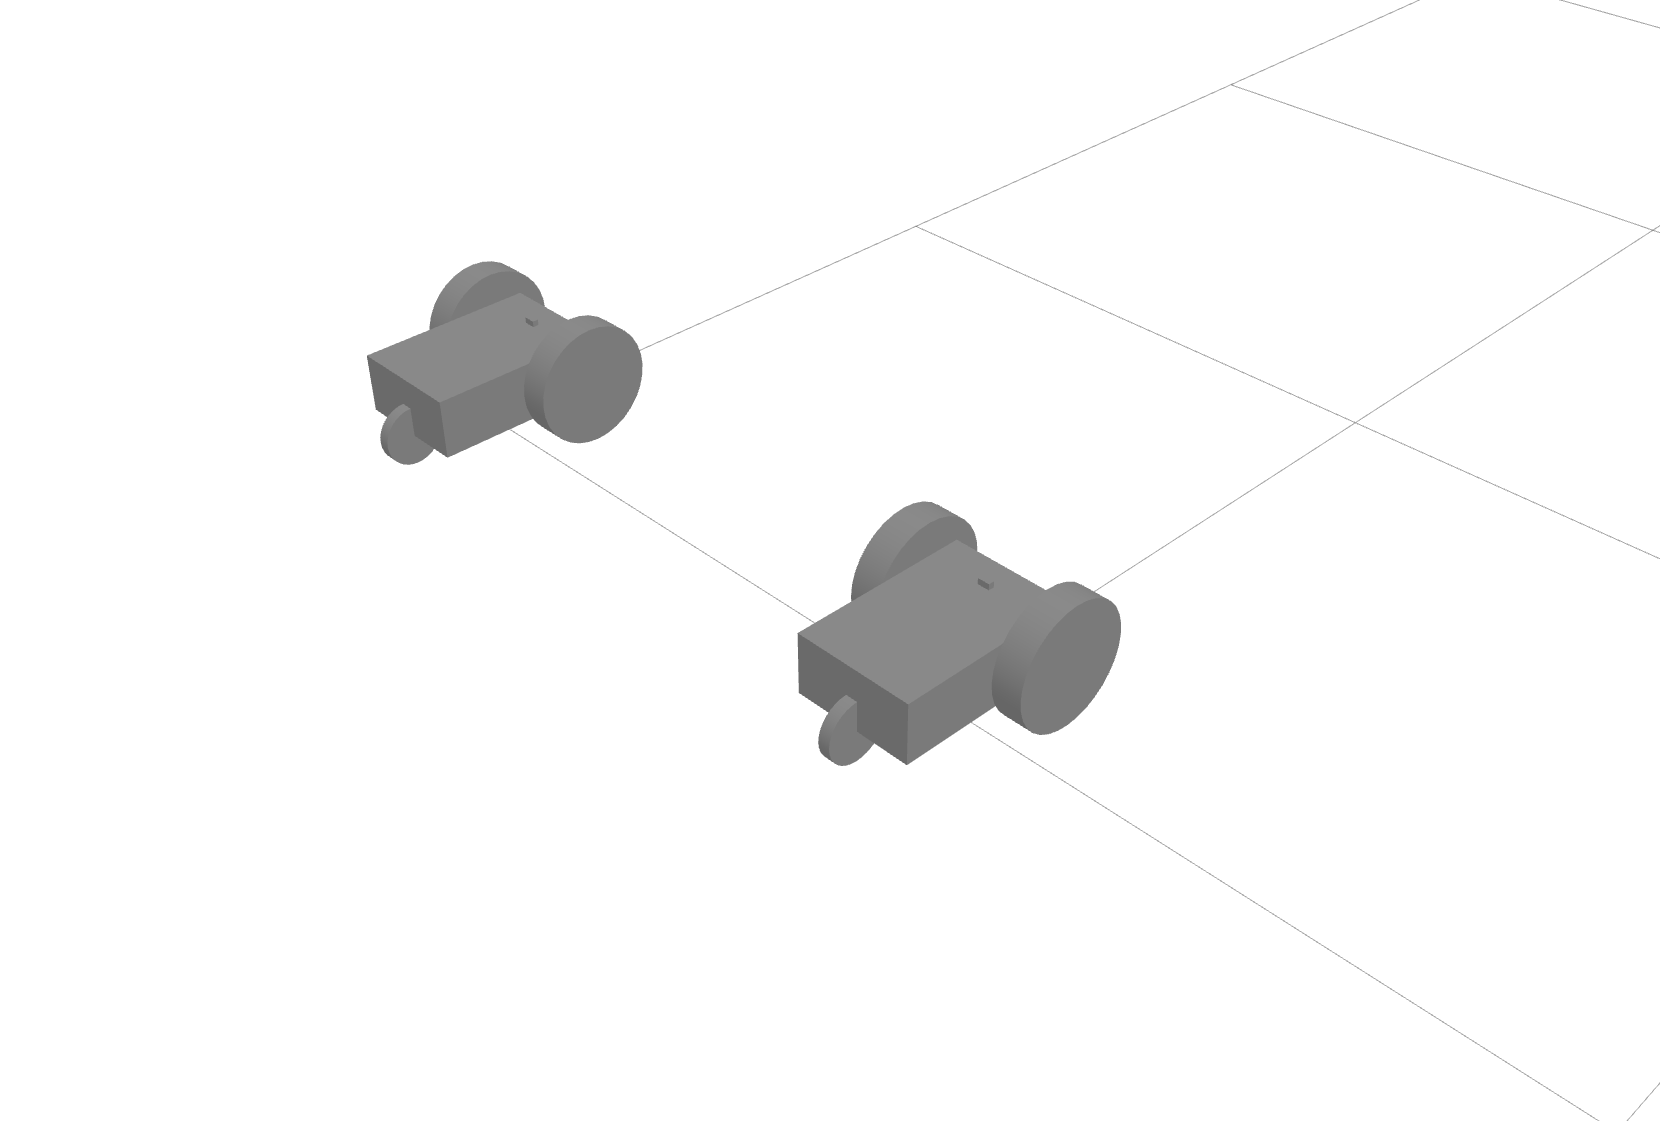
\includegraphics[width=0.5\textwidth]{graphics/crawlers.png}
				\caption{Modèle de crawler utilisé pour l'inspection acoustique de structures métalliques.}
				\label{fig:crawler}
			\end{figure}

			Chaque robot est soit émetteur, soit récepteur, soit les deux.
			Les crawlers sont équipés de différents capteurs.
			Parimi eux:
			\begin{itemize}
				\item un capteur IMU (Inertial Measurement Unit)
				\item un capteur UGW (Ultrasonic Guided Waves)
				\item un capteur LIDAR (Light Detection And Ranging)
			\end{itemize}
			Le capteur IMU permet de connaître l'orientation du robot dans l'environnement.
			Le capteur UGW permet de détecter les zones de corrosion sur la surface métallique en émettant et en recevant des ondes ultrasoniques.
			Le capteur LIDAR permet de détecter les obstacles dans l'environnement.
			Les obstacles considérés ici, sont principalement les différents robots inspectant la surface métallique.
			La détection de ces zones de corrosion est réalisée par l'émission d'ondes ultrasoniques par un robot et la réception de ces ondes par un autre robot.
			Dans la mesure où l'onde reçu par un des crawler est altérée, alors il existe un point de corrosion entre le robot émetteur et le robot récepteur.
			La détection de ces zones de corrosion est réalisée en temps réel.
			La portée maximale des ondes ultrasoniques est notée $d_{max}$.
			Nous approximons le temps de propagation des ondes ultrasoniques dans la surface métallique par un temps nul.

			Nous utilisons une grille d'occupation pour modéliser l'environnement dans lequel les robots évoluent lors de l'inspection acoustique des structures métalliques.
			Cette grille nous permet de représenter et de catégoriser les différents états des zones de la surface métallique.
			La grille d'occupation est composée de cellules, où chaque cellule correspond à une petite région de l'environnement.
			En particulier, nous avons utilisé une résolution de 0.05 mètre par cellule.
			Nous utilisons trois états pour caractériser ces cellules : inconnu, vide et occupé.
			L'état inconnu désigne les zones dont l'état n'a pas encore été déterminé ou détecté.
			L'état vide indique les zones où il n'y a pas de corrosion détectée, c'est-à-dire que la surface métallique est saine.
			Enfin, l'état occupé représente les zones de corrosion identifiées, où la présence de défauts ou de détérioration est détectée.

			En utilisant cette grille d'occupation, nous pouvons suivre et mettre à jour en temps réel l'état des différentes zones de la surface métallique pendant l'inspection.
			Cela nous permet de planifier les mouvements des robots, d'optimiser leur trajectoire et d'assurer une couverture complète de la surface à inspecter.
			De plus, cette représentation nous offre une vision claire de l'état de corrosion de la structure métallique, facilitant ainsi l'analyse et l'évaluation des résultats de l'inspection.

			Dans la suite de notre proposition, nous détaillerons les algorithmes et les méthodes utilisées pour mettre à jour la grille d'occupation en fonction des informations recueillies par les capteurs des robots.
			Nous discuterons également des stratégies de navigation multi-robots qui exploitent cette modélisation pour optimiser l'acquisition de données et améliorer l'efficacité de l'inspection acoustique.
		\subsection{Proposition de solution}
			Nous présentons notre proposition de solution pour l'inspection acoustique de structures métalliques en utilisant des stratégies de navigation multi-robots.
			Nous avons développé trois stratégies spécifiques pour optimiser l'acquisition de données et permettre la réalisation de la tomographie des surfaces métalliques.
			\subsubsection*{Stratégie de navigation \textit{peinture au rouleau}}
				La première stratégie de navigation que nous proposons est la stratégie de navigation \textit{peinture au rouleau}.
				Cette stratégie repose sur une exploration grossière de la surface à inspecter, où les robots se déplacent en ligne droite sur des trajectoires parallèles, garantissant une couverture globale de la zone d'inspection.
				Il s'agit donc ici d'effectuer un quadrillage de la surface à inspecter.

				\begin{figure}[h!]
					\centering
					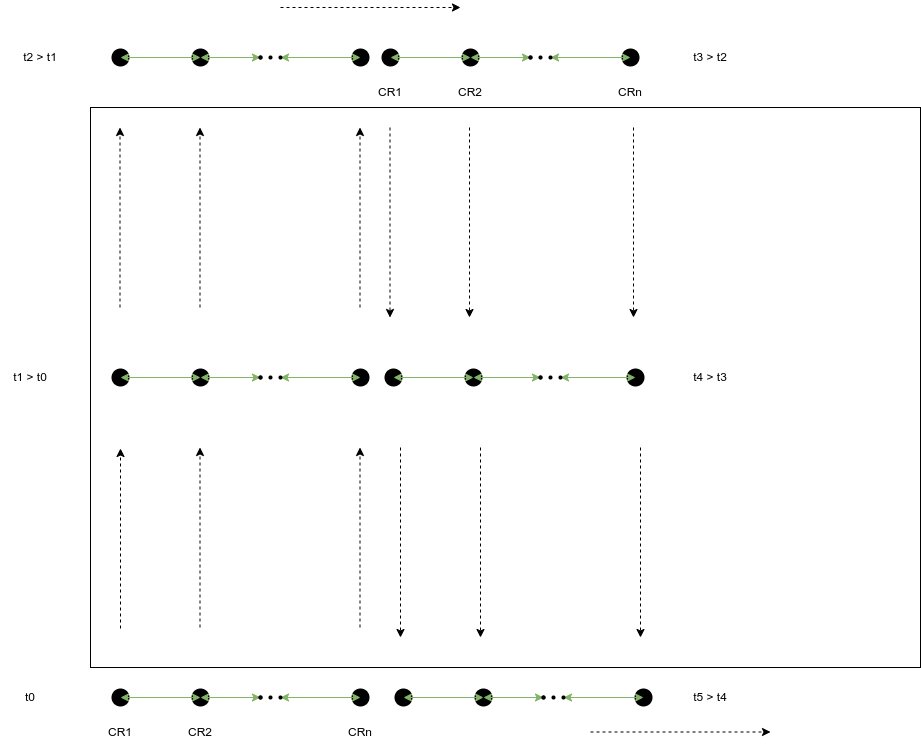
\includegraphics[scale=0.5]{graphics/peinture_au_rouleau1.png}
					\caption{Stratégie de navigation peinture au rouleau.}
					\label{fig:peinture_au_rouleau1}
				\end{figure}

				Nous présentons à la figure~\ref{fig:peinture_au_rouleau1} un schéma décrivant la stratégie de navigation peinture au rouleau.
				Cette stratégie consiste en deux phases, une phase de déplacement vertical et une phase de déplacement horizontal.
				La figure~\ref{fig:peinture_au_rouleau1} présente la première phase de déplacement vertical.
				Afin de réaliser cette stratégie, un minimum de $n \ge 2$ robots, aligné horizontalement et séparé par une distance $d$, est utilisé.
				Ces robots se déplacent verticalement, en simulatané, en suivant une tarjectoire parallèle.
				Une fois l'extrémité de la surface à inspecter atteinte, les robots effectuent une rotation de 90 degrés et se translatent horizontalement, en simulatané, d'une distance $2 * d$.
				Ils effectuent ensuite une nouvelle rotation de 90 degrés et se déplacent de nouveau verticalement, en ligne droite, en simulatané, en suivant une trajectoire parallèle entre eux, jusqu'à atteindre l'autre extrémité de la surface à inspecter.
				Ce procédé est répété jusqu'à ce que la surface métallique soit entièrement inspectée.
				Le même procédé est ensuite répété, mais cette fois-ci, horizontalement.

				Le fait que les robots se déplacent en suivant une trajectoire parallèle et en simulatané, implique que les rayons du signal émit par le robot émetteur et reçu par le robot récepteur, ont toujours une orientation de $0$ pour la phase verticale et une orientation de $\frac{\pi}{2}$ pour la phase horizontale.
				Il n'y a donc pas une grande variation de l'orientation du signal émis et reçu.
				Ainsi, cette stratégie ne pourra approcher les enveloppes convexes des zones de corrosion que par des rectangles.
			\subsubsection*{Stratégie de navigation \textit{ski nordique}}
				La deuxième stratégie que nous proposons est la stratégie de navigation \textit{ski nordique}.
				Cette stratégie consiste toujours en des déplacements en ligne droite et en suivant des trajectoires parallèle, mais cette fois-ci, les robots se déplacent de manière séquentielle et non plus de manière simulatanée.
				Dans cette stratégie, nous avons voulu accroître la diversité d'orientation des rayons du signal émis et reçu, afin d'approcher plus précisément les enveloppes convexes des zones de corrosion.

				\begin{figure}[h!]
					\centering
					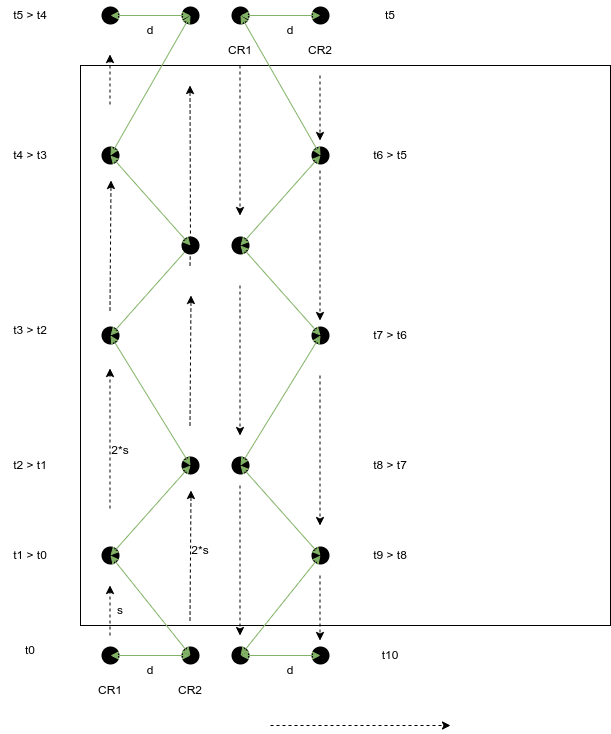
\includegraphics[scale=0.5]{graphics/ski_nordique.png}
					\caption{Stratégie de navigation ski nordique.}
					\label{fig:ski_nordique1}
				\end{figure}

				La figure~\ref{fig:ski_nordique1} présente un schéma décrivant la stratégie de navigation \textit{ski nordique}.
				Cette stratégie consiste également en deux phases, une phase de déplacement vertical et une phase de déplacement horizontal.
				La figure~\ref{fig:ski_nordique1} présente la première phase de déplacement vertical.
				Afin de réaliser cette stratégie, un minimum de $n \ge 2$ robots, aligné horizontalement et séparé par une distance $d$, est utilisé.
				Par soucis de clarté, nous avons représenté à la figure~\ref{fig:ski_nordique1} uniquement deux robots.
				Ces robots se déplacent verticalement, en suivant une trajectoire parallèle, mais de manière séquentielle.
				Le premier robot se déplace en ligne droite d'une distance $s$ et s'arrête.
				Le second robot se déplace ensuite en ligne droite d'une distance $2 * s$ et s'arrête.
				Ce procédé est répété jusqu'à ce que la l'extrémité de la surface soit atteinte.
				Ensuite les robots répètent ce même procédé, dans le sens inverse et de manière à ce que les points d'arrêt des robots ne soient pas les mêmes que ceux précédemment.
				Les robots se déplacent ensuite horizontalement d'une distance $d$ et répètent le même procédé jusqu'à ce que la surface métallique soit entièrement inspectée.
				Le même procédé est ensuite répété, mais cette fois-ci, horizontalement.

				Le fait que les robots se déplacent en suivant une trajectoire parallèle, mais de manière séquentielle, implique que les rayons du signal émit par le robot émetteur et reçu par le robot récepteur, ont une orientation d'une plus grande variation.
				Ainsi, cette stratégie permet d'approcher les enveloppes convexes des zones de corrosion par des formes plus diverses et précises que des rectangles.
			\subsubsection*{Stratégie de navigation \textit{investigation polygonale}}
				La troisième stratégie que nous proposons est la stratégie de navigation \textit{investigation polygonale}.
				Nous avons vu,  précédemment, qu'à l'issue de la réalisation de la stratégie de navigation \textit{peinture au rouleau}, l'enveloppe convexe des zone de corrosion est approximée par un rectangle.
				Cette approximation est un peut plus précise pour la stratégie de navigation \textit{ski nordique}.
				Il serait intéréssant de pouvoir un plus grand degré de précision autours des zones potentielles de corrosion.
				C'est ce que nous proposons avec la stratégie de navigation \textit{investigation polygonale}.
				Cette stratégie consiste à investiguer autour des zones potentielles de corrosion, détectées au préalable par une des deux stratégies de navigation précédentes.
				Elle consiste à positioner les robots autours des zones de corrosion et à les faire se déplacer en suivant une trajectoire polygonale, de manière à ce que les rayons du signal émis et reçu aient une orientation d'une plus grande variation autour même de ces zones.

				\begin{figure}[h!]
					\centering
					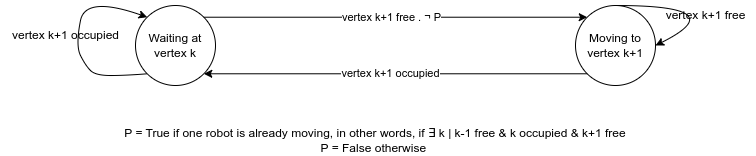
\includegraphics[scale=0.6]{graphics/automat_poly.png}
					\caption{Stratégie de navigation investigation polygonale.}
					\label{fig:automat}
				\end{figure}

				Nous présentons à la figure~\ref{fig:automat} un automate à états finis décrivant la stratégie de navigation \textit{investigation polygonale}.
				Au début de la stratégie de navigation \textit{investigation polygonale}, les $n \in \mathbb{N}$ robots constitutifs de $k \in \mathbb{N}$ équipes sont positionnés sur des somets consécutifs d'un polygone englobant la zone potentielle de corroion.
				Dans cette dernière, chaque robot a deux états.
				Le premier consiste à attendre et le second consiste à se déplacer en suivant la trajectoire polygonale, à savoir parcourir les différents sommets constituant le polygone.
				Le robot capable d'avancé, c'est-à-dire, dont le sommet suivant n'est pas occupé par un autre robot, avance.
				Les autres attendent jusqu'à ce que le robot qui avance atteigne le dernier sommet libre du polygone.
				Le procédé est ensuite répété pour chaque robot de chaque équipe jusqu'à ce que les sommets occupés par les robots soient les mêmes que ceux occupés au début de la stratégie de navigation \textit{investigation polygonale}.

				Cette stratégie a deux avantages.
				Le premier est qu'elle permet de rapidement éliminer les zones fantômes.
				Le second est qu'elle permet d'approcher les enveloppes convexes des zones de corrosion par des formes plus diverses et précises que des rectangles du fait de la grande variation de l'orientation des rayons du signal émis et reçu par les robots autour de chaque sommet du polygone.

				Cette stratégie nécéssite deux étapes préalables à son exécution :
				\begin{enumerate}
					\item l'extraction des zones de corrosion détectées par une des stratégies de navigation précédentes.
					\item la détermination de l'ordre d'investigation des zones de corrosion.
				\end{enumerate}

				La première étape peut être résolue en utilisant un algorithme de décomposition de graphe en composantes fortement connexes.
				Une composante fortement connexe est définie à la définition~\ref{def:scc}.
				Nous considérons alors notre image comme un graphe non orienté $G = (V, E)$, où  $V$ est l'ensemble des sommets du graphe, correspondant aux pixels de l'image et $E$ sont les arêtes du graphe, correspond aux pixels adjacents.
				Ce problème est bien connu et il existe des algorithmes simples pour les résoudre comme l'algorithme de Tarjan de compléxité temporelle linéaire $O(|V| + |E|)$.
				Nous ne nous pencherons pas plus sur ce problème et confions sa résolution à la bibliothèque OpenCV.

				\begin{Definition}[Composante fortement connexe (SCC)]
					\label{def:scc}
					Une composante fortement connexe d'un graphe orienté $G = (V, E)$ est un sous-ensemble $C$ de $V$ tel que pour tout couple de sommets $(u, v) \in C^2$, il existe un chemin de $u$ à $v$ et un chemin de $v$ à $u$.
				\end{Definition}

				La seconde étape peut être résolue en utilisant un algorithme de TSP (\textit{Travelling Salesman Problem}) dans le cas où le nombre d'équipe $k = 1$ et un algorithme de mTSP (\textit{(multiple depot) multiple Travelling Salesman Problem}) dans le cas où le nombre d'équipe $k > 1$.
				Il existe plusieurs paradigmes de résolution pour résoudre ce genre de problème.
				Un premier est de trouver une solution exacte en utilisant un algorithme de programmation linéaire en nombres entiers.
				Un second est de trouver une solution approchée en utilisant une méta-heuristique.

				\begin{Definition}[Problème du voyageur de commerce (TSP)]
					\label{def:tsp}
					Étant donné une liste de villes et les distances entre chaque paire de villes, quel est l'itinéraire le plus court possible qui visite chaque ville exactement une fois et revient à la ville d'origine ?
				\end{Definition}

				Le problème du voyageur de commerce est un problème NP-complet et il peut être traité comme un problème d'optimisation linéaire en nombres entiers.
				Pour ce faire, nous utilisons la formulation présentée à l'équation~\ref{eq:tsp}.

				\begin{equation}
					\label{eq:tsp}
					\begin{array}{ll@{}ll}
						\text{minimiser}  & \displaystyle\sum\limits_{i \in V} \sum\limits_{j \in V} c_{ij} x_{ij} \\
						\text{soumis à}   & \displaystyle\sum\limits_{i \in V} x_{ij} = 1 & \forall j \in V\\
						& \displaystyle\sum\limits_{j \in V} x_{ij} = 1 & \forall i \in V\\
						& \displaystyle\sum\limits_{i \in S} \sum\limits_{j \in S} x_{ij} \leq |S| - 1 & \forall S \subset V, 2 \leq |S| \leq |V| - 1\\
						& x_{ij} \in \{0, 1\} & \forall i \in V, \forall j \in V\\
					\end{array}
				\end{equation}

				La fonction objectif à minimiser de la formulation~\ref{eq:tsp} est la somme des distances entre chaque paire de villes.
				Les deux premières contraintes assurent que chaque ville est visitée exactement une fois.
				La troisième contrainte assure que le cycle formé par les villes visitées est simple, c'est-à-dire, qu'il ne contient pas de sous-cycles.
				La dernière contrainte assure que les variables de décision $x_{ij}$ sont binaires, avec $x_{ij} = 1$ si le robot se déplace de la ville $i$ à la ville $j$ et $x_{ij} = 0$ sinon.

				\begin{Definition}[Problème du voyageur de commerce multiple avec dépots multiples (mTSP)]
					\label{def:mtsp}
					Étant donné une liste de villes et les distances entre chaque paire de villes, quel est l'itinéraire le plus court possible qui visite chaque ville exactement une fois et revient à la ville d'origine, en considérant que l'on a $k \in \mathbb{N}$ voyageurs ?
				\end{Definition}

				Le problème du voyageur de commerce multiple avec dépots multiples est également un problème NP-complet.
				Celui-ci peut être résolu en utilisant une méta-heuristique comme un algorithme génétique~\cite{SinghMTSP, Kiraly2011}

				Dans les prochaines sections, nous détaillerons chaque stratégie de navigation, en exposant les algorithmes et les mécanismes spécifiques utilisés pour mettre en œuvre notre proposition de solution. Nous analyserons également les performances et les résultats obtenus à travers des expérimentations et des évaluations approfondies.
		\subsection{Étude théorique de propriétés de la solution proposée}
			\subsubsection*{Stratégie de navigation \textit{ski nordique}}
				\begin{Proposition}
					L'angle du signal émis et reçu par les robots, pour la stratégie de navigation \textit{ski nordique}, varie entre $-\tan^{-1}(\frac{s}{d})$ et $\tan^{-1}(\frac{s}{d})$.
					\label{prop:angle_ski_nordique}
				\end{Proposition}
				\begin{proof}
					Pour démontrer la proposition~\ref{prop:angle_ski_nordique}, nous nous appuyons sur les propriétés de trigonométrie.
					Nous explicitons à la figure~\ref{fig:angle_ski_nordique} la démarche entreprise pour trouver $\alpha = -\tan^{-1}(\frac{s}{d})$

					\begin{figure}[h!]
						\centering
						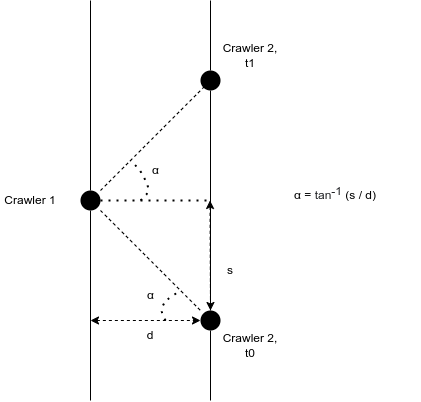
\includegraphics[scale=0.5]{graphics/angle_ski_nordique.png}
						\caption{Angle du signal émis et reçu pour la stratégie de navigation ski nordique.}
						\label{fig:angle_ski_nordique}
					\end{figure}
				\end{proof}
			\subsubsection*{Stratégie de navigation \textit{investigation polygonale}}
				\begin{Proposition}
					L'enveloppe convexe des zones de corrosion à l'issue de l'investigation polygonale, avec un polygone à $p$ sommets, $p \in \mathbb{N}$, est un polygone d'au plus $2p$ sommets.
					\label{prop:cotes_poly}
				\end{Proposition}
				\begin{proof}
					Démontrons la proposition~\ref{prop:cotes_poly}.
					\begin{itemize}
						\item On a, pour chaque sommet du polygone, il existe deux droites passant par ce point et touchant la zone de corrosion sans la traverser.
						\item On a donc pour un sommet du polygone, au plus deux droites qui participent à la construction de l'enveloppe convexe et donc, dont un segement de ces droites est une arête de l'enveloppe convexe.
						\item On a donc pour un sommet du polygone, au plus deux arêtes de l'enveloppe convexe.
						\item On a donc pour un polygone à $p$ sommets, au plus $2p$ arêtes de l'enveloppe convexe.
						\item On a donc pour un polygone à $p$ sommets, au plus $2p$ sommets de l'enveloppe convexe.
					\end{itemize}
				\end{proof}

				\begin{Proposition}
					\TODO{Qu'est ce que je souhaite démontrer ?}
					\label{prop:}
				\end{Proposition}
				\begin{proof}
					Démontrons la proposition~\ref{prop:}.
					\TODO{Faire la preuve.}
				\end{proof}
	\section{Implémentations techniques}
		Dans cette section, nous mettons en évidence certaines des différentes implémentations techniques que nous avons développées pour soutenir nos solutions de navigation et de contrôle multi-robots dans le contexte de l'inspection acoustique de structures métalliques.
		Nous commençons par décrire notre adaptation de l'algorithme de tracé de sagement de Bresenham, largement utilisé pour déterminer quels sont les points d'un plan discret qui doivent être tracés afin de former une approximation de segment de droite entre deux points donnés.
		Ensuite, nous abordons l'implémentation de l'algorithme \textit{peinture au rouleau}, qui permet aux robots de se déplacer de manière simultanée, en suivant des trajectoires parallèles.
		Nous poursuivons avec l'implémentation de l'algorithme \textit{ski nordique}, qui permet aux robots de se déplacer de manière alternée, en suivant des trajectoires parallèles, modifiant ainsi l'orientation du vecteur représentant la direction de déplacement de l'onde émise et reçue par la paire de robot.
		De plus, nous examinons l'implémentation de l'algorithme \textit{investigation polygonale}, qui permet aux robots d'examiner plus précisément des zones suspectes de corrosion.
		Enfin, nous présentons l'algorithme de calcul du $\kappa$ de Cohen, utilisé pour évaluer la qualité et la fiabilité des résultats de l'inspection acoustique.
		Nous discutons en détail de notre implémentation de cet algorithme, qui fournit des mesures quantitatives pour évaluer la performance des robots dans l'inspection des structures métalliques.
		Chacune de ces implémentations techniques contribue à l'efficacité et à la précision de notre approche de navigation et de contrôle multi-robots, et sera examinée en détail dans les sous-sections suivantes.
		\subsection*{Algorithme de tracé de segement de Bresenham}
			L'algorithme de tracé de segment de Bresenham est couramment utilisé pour déterminer les points d'un plan discret qui doivent être tracés afin de former une approximation de segment de droite entre deux points donnés.
			Lors du balaiement de la surface à inspecter par une paire de robot émetteur et récepteur, le robot émetteur émet une onde acoustique dans la structure métallique, qui est ensuite reçue par le robot récepteur.
			La détection étant considérée comme parfaite, le robot récepteur reçoit l'onde émise par le robot émetteur, sans quasi altération de la puissance du signal, si et seulement si le segment de droite entre les deux robots ne traverse pas une zone de corrosion.
			Il est ainsi possible de déterminer si une zone de corrosion est présente entre les deux robots en vérifiant si le signal reçu par le robot récepteur est suffisamment puissant.
			Dans la mesure où il n'y a pas de détection de corrosion entre l'émetteur et le récepteur, alors le segment de droite entre les deux robots est considéré comme étant libre de corrosion.
			Dans le cas contraire, alors les points du segment de droite entre les deux robots sont considérés comme étant de la corrosion, à l'exception des points préalablement perçu comme étant libre de corrosion.

			\begin{algorithm}[h!]
				\caption{Processus de mise à jour de la grille d'occupation à l'aide de l'algorithme de tracéde segment de Bresenham.}
				\label{alg:Bresenham}
				\KwData{$P_1 \in \mathbb{R}^2$, $P_2 \in \mathbb{R}^2$, $pw \in \mathbb{R}$, $threshold \in \mathbb{R}$, $G$: $l \times w \rightarrow [\text{UNKNOWN}, \text{EMPTY}, \text{OCCUPIED}]$, $l \in \mathbb{N}$, $w \in \mathbb{N}$ \\
					with $P_1$ and $P_2$ the two points to connect, $pw$ the power of the UGW, $threshold$ the threshold above which the power of the UGW is considered undistributed and $G$ the grid to update.}
				\KwResult{The updated grid.}
				$p_0 \gets \text{from\_position\_to\_grid\_coordinate}(P_1)$ \\
				$p_1 \gets \text{from\_position\_to\_grid\_coordinate}(P_2)$ \\
				\If{\text{is\_out\_of\_grid}($p_0$) \textbf{or} \text{is\_out\_of\_grid}($p_1$)}{
					\Return
				}
				$dx \gets p_1.x - p_0.x$ \\
				$dy \gets p_1.y - p_0.y$ \\
				$sx \gets \text{sign}(dx)$ \\
				$sy \gets \text{sign}(dy)$ \\
				$err = dx - dy$ \\
				\While{$p_0 \neq p_1$}{
					\If{$pwd \leq threshold$ \textbf{and} $G(p_0) = \text{UNKNOWN}$}{
						$G(p_0) \gets \text{OCCUPIED}$
					}
					\ElseIf{$pwd > threshold$}{
						$G(p_0) \gets \text{EMPTY}$
					}
					$e2 \gets 2 \times err$ \\
					\If{$e2 > -dy$}{
						$err \gets err - dy$ \\
						$p_0.x \gets p_0.x + sx$
					}
					\If{$e2 < dx$}{
						$err \gets err + dx$ \\
						$p_0.y \gets p_0.y + sy$
					}
				}
			\end{algorithm}

			Nous utilisons donc l'algorithme de tracé de segment de Bresenham pour déterminer les points du segment de droite entre les deux robots.
			L'algorithme est présenté à l'algorithme~\ref{alg:Bresenham}. La partie adaptée à notre problème se trouve entre les lignes 12 et 17 de ce dernier.
			À cet endroit, nous verrifions si la puissance du signal est suffisamment altérée et si le point du segment de droite entre les deux robots n'a pas déjà été perçu comme étant libre de corrosion.
			Si c'est le cas, alors le point considéré est marqué comme étant de la corrosion, modélisé par la valeur \texttt{OCCUPIED}.
			Si la puissance du signal n'est pas suffisamment altérée, alors le point considéré est marqué comme étant libre de corrosion, modélisé par la valeur \texttt{EMPTY}.
			Une fois que tous les points du segment ont été parcourus, la grille $G$ est mise à jour avec les nouvelles informations.
			L'algorithme de tracé de segment de Bresenham contribue ainsi à la construction de la grille d'occupation qui permet de localiser les zones de corrosion détectées par les robots lors de l'inspection acoustique des structures métalliques.
		\subsection*{Algorithme \textit{peinture au rouleau} et \textit{ski nordique}}
			Nous présentons dans cette sous-section les implémentations des algorithmes \textit{peinture au rouleau} et \textit{ski nordique}, présentées en annexe~\ref{annexe:implementations}, au listing~\ref{lst:peinture_au_rouleau} et au listing~\ref{lst:ski_nordique}.

			L'implémentation de ces algorithmes, ont été réalisées en utilisant le langage de programmation Python et les bibliothèques ROS (Robot Operating System).
			Dans ces implémentations, nous utilisons le framework Task Manager~\cite{ROSTaskManager} pour gérer les tâches des robots inspecteurs.
			Tout d'abord, nous initialisons le nœud ROS et créons un client de tâches.
			Ensuite, nous récupérons les paramètres nécessaires tels que la vitesse des crawlers, l'identifiant du crawler, la distance entre les crawlers, le chevauchement ou encore les dimensions de la surface à inspecter.

			Les algorithmes sont ensuite exécutés en suivant une séquence de mouvements précis.
			Pour chaque crawler, nous définissons des trajectoires verticales et horizontales en utilisant une boucle itérative et des calculs mathématiques. Les crawlers se déplacent le long des trajectoires définies, en utilisant les fonctions du client de tâches telles que \texttt{AlignWithTarget} et \texttt{FollowLine} pour maintenir une trajectoire précise.

			Pendant l'exécution des algorithmes, les crawlers se synchronisent en utilisant les fonctions \texttt{SetStatusSync} et \texttt{WaitForStatusSync} du client de tâches.
			Cela garantit que les crawlers exécutent les mouvements de manière coordonnée et se positionnent correctement pour couvrir toute la surface métallique.
			À la fin de chaque étape de mouvement, le statut est mis à jour et la synchronisation est effectuée avec le partenaire correspondant.

			L'implémentation des deux algorithmes \textit{peinture au rouleau} et \textit{ski nordique} permettent aux crawlers d'inspecter la surface métallique de manière méthodique et complète.
			En utilisant des trajectoires verticales et horizontales, les crawlers parcourent la surface en chevauchant les zones précédemment inspectées pour s'assurer d'une couverture optimale.
			Ici, nous avons utilisé un chevauchement de 10 cm entre les différentes trajectoires verticales et horizontales.

			Une fois les algorithmes terminés, le temps d'exécution est enregistré, fournissant une indication de la durée nécessaire pour inspecter la surface métallique.
			La grille d'occupation est également enregistré afin de calculer le score de l'inspection.
			Cette implémentation constitue une étape essentielle dans notre proposition de solution pour l'inspection acoustique de structures métalliques et permet de garantir une couverture complète et efficace de la surface à inspecter.
		\subsection*{Algorithme \textit{investigation polygonale}}
			Nous présentons dans cette sous-section l'implémentation de l'algorithme \textit{investigation polygonale}, présentée en annexe~\ref{annexe:implementations}, au listing~\ref{lst:investigation_polygonale}.

			L'implémentation de cet algorithme, a également été réalisée en utilisant le langage de programmation Python et les bibliothèques ROS (Robot Operating System).
			Dans cette implémentation, nous utilisons toujours le framework Task Manager~\cite{ROSTaskManager} pour gérer les tâches des robots inspecteurs.
			Premièrement, nous initialisons le nœud ROS et récupérons les différents paramètre et plus particulièrement la carte des zones potentielles et grossières de corrosion, sur laquelle nous nous basons pour l'inspection.
			Ensuite nous extrayons les composantes fortement connexes de la carte en utilisant la fonction \texttt{connectedComponentsWithStats} de la biblliothèque d'OpenCV.
			Cette fonction utilise l'algorithme spaghetti de Bolleli~\cite{BolelliSpaghetti} pour extraire les composantes fortement connexes d'une image.
			Pour chacune de ces composantes nous récupérons son centre et ses dimensions.
			Ensuite, nous construisons un polygone à $p \in \mathbb{N}$ côtés autour de chaque centre d'une composante.
			Pour ce faire nous plaçons $p$ sur une ellipse centrée sur le centre de la composante et dont les axes sont les dimensions de la composante.
			Nous avons donc pour chaque zone potentielle de corrosion un polygone à $p$ côtés qui l'entoure.
			Il ne reste plus qu'à trouver le plus court chemin qui passe par tous les polygones.
			Pour cela, nous utiilisons la bibliothèque Gurobi pour résoudre un simple TSP dans le cas où le nombre d'équipe de robots $k = 1$.
			Lorsque $k > 1$, nous utilisons l'algorithme génétique proposé par Elad Kivelevitch~\cite{MDMTSPV_GA} pour résoudre le problème du mTSP avec plusieurs dépôts.

			\TODO{investigation}
		\subsection*{Algorithme de calcul du $\kappa$ de Cohen}
			L'évaluation de la qualité et de la fiabilité des résultats de l'inspection acoustique est essentielle pour garantir des mesures précises de l'état des structures métalliques.
			Dans cette sous-section, nous présentons l'algorithme du calcul du $\kappa$ de Cohen, présenté à l'algorithme~\ref{alg:Cohen_Kappa}, une mesure statistique couramment utilisée pour évaluer l'accord entre les résultats obtenus par les robots et une référence humaine.

			\begin{algorithm}[h!]
				\caption{Algorithme du $\kappa$ de Cohen.}
				\label{alg:Cohen_Kappa}
				\KwData{$I_0$: $l \times w \times 3 \rightarrow [0 .. 255]$, $I$: $l \times w \times 3 \rightarrow [0 .. 255]$, $l \in \mathbb{N}$, $w \in \mathbb{N}$ \\
					with $I_0$ the ground truth image and $I$ the image to score.}
				\KwResult{$\kappa \in [0, 1]$}
				$TP \gets 0$ \\
				$TN \gets 0$ \\
				$FP \gets 0$ \\
				$FN \gets 0$ \\
				\For{$i \gets 1$ \KwTo $l$}{
					\For{$j \gets 1$ \KwTo $w$}{
						\If{$\text{is\_label\_1}(I_0(i, j))$}{
							\If{$\text{is\_label\_1}(I(i, j))$}{
								$TP \gets TP + 1$
							}
							\Else{
								$FN \gets FN + 1$
							}
						}
						\Else{
							\If{$\text{is\_label\_1}(I(i, j))$}{
								$FP \gets FP + 1$
							}
							\Else{
								$TN \gets TN + 1$
							}
						}
					}
				}
				$f_c \gets \frac{(TN + FN) (TN + FP) + (FP + TP) (FN + TP)}{TP + TN + FN +FP}$ \\
				$\kappa \gets \frac{TP + TN - f_c}{TP + TN + FN + FP - f_c}$
			\end{algorithm}

			L'algorithme de calcul du $\kappa$ de Cohen se base sur la notion de concordance et de discordance entre les résultats des inspections réalisées par les robots et celles réalisées par des inspecteurs humains.
			Il prend en compte les résultats positifs, négatifs, faux positifs et faux négatifs obtenus lors de l'inspection acoustique.
			Ces informations sont utilisées pour calculer la valeur du coefficient de Cohen, noté $\kappa$, avec $\kappa = \frac{p_o - p_e}{1 - p_e}$, où $p_o$ est le taux d'accord observé et $p_e$ le taux d'accord attendu.

			L'algorithme se déroule en plusieurs étapes.
			Tout d'abord, les résultats des inspections réalisées par les robots et réel répartition des zones de corrosion sont comparés pour chaque zone inspectée.
			Ensuite, les résultats sont regroupés en quatre catégories : concordance positive, concordance négative, discordance positive (faux positifs) et discordance négative (faux négatifs).
			Ces catégories sont utilisées pour calculer les taux d'observation et d'accord observés entre les robots et la véritable répartition des zones de corrosion.
			Le $\kappa$ de Cohen est ensuite calculé à partir des taux d'observation et d'accord observés, prenant en compte la possibilité de concordance due au hasard.
			Plus le $\kappa$ de Cohen se rapproche de 1, plus il y a un accord élevé entre les résultats des robots et ceux des inspecteurs humains.
			En revanche, un $\kappa$ proche de 0 indique un faible niveau d'accord, tandis qu'un $\kappa$ négatif suggère une discordance entre les résultats.
			Une Interprétation du $\kappa$ de Cohen selon Landis et Koch est présentée dans le tableau~\ref{tab:Kappa_Cohen}.

			\begin{table}[h!]
				\centering
				\begin{tabular}{|c|c|}
					\hline
					$\kappa$ & Interprétation \\
					\hline
					$< 0$ & Désaccord \\
					\hline
					$0.00 - 0.20$ & Accord très faible \\
					\hline
					$0.21 - 0.40$ & Accord faible \\
					\hline
					$0.41 - 0.60$ & Accord modéré \\
					\hline
					$0.61 - 0.80$ & Accord fort \\
					\hline
					$0.81 - 1.00$ & Accord presque parfait \\
					\hline
				\end{tabular}
				\caption{Interprétation du $\kappa$ de Cohen selon Landis et Koch.}
				\label{tab:Kappa_Cohen}
			\end{table}

			Nous avons implémenté cet algorithme dans le cadre de notre projet, en utilisant les résultats des inspections acoustiques effectuées par les robots et des cartes composées de zones de corrosion comme base de comparaison.
			Cette implémentation nous permet d'obtenir des mesures quantitatives pour évaluer la performance de notre approche de navigation et de contrôle multi-robots dans l'inspection des structures métalliques.
			Dans les prochaines sections, nous détaillerons les résultats obtenus grâce à l'application de cet algorithme du calcul du $\kappa$ de Cohen.
	\section{Expérimentations, validations et évaluations}
		Dans cette section, nous présentons les expérimentations que nous avons menées pour valider et évaluer nos différentes stratégies de navigation et de contrôle multi-robots dans le contexte de l'inspection acoustique de structures métalliques.
		Ces expérimentations visent à démontrer l'efficacité, la précision et la fiabilité de notre système dans la détection et la localisation des zones de corrosion.

		Pour mener à bien ces étapes, nous avons choisi d'effectuer nos expériences en utilisant Gazebo, un environnement de simulation bien établi dans le domaine de la robotique.
		Nous avons commencé par construire plusieurs cartes de tests.
		Ces cartes modélisent une surface plane sur laquelle sont placées des formes géométriques simples, des rectangles et des cercles, et des formes plus complexes, des polygones entre 3 et 8 sommets.
		Ces différentes formes géométriques représentent les zones de corrosion que nous souhaitons détecter et localiser.
		Nous présentons en annexe~\ref{annexe:cartes}, à la figure~\ref{fig:test_models} les cartes que nous avons construites pour nos expérimentations.
		Chacune de ces cartes est de taille 6 mètres par 6 mètres.
		Le nombre de zones de corrosion varie entre 5, 8, 11, 15, 20 et 30 zones.
		La taille et l'emplacement des zones de corrosion sont générés aléatoirement.
		Pour les cartes de 5, 8, 11 et 15 zones, nous avons généré 5 cartes différentes afin d'avoir des résultats plus représentatifs.
		Nous ne nous sommes pas permis de générer plusieurs cartes pour les cartes de 20 et 30 zones, le temps d'investigation polygonale étant trop conséquent.

		Nous avons également simulé le capteur UGW par un capteur Ultra wideband (UWB).
		Ce capteur UWB permet d'émettre une impulsion et de la recevoir.
		En mesurant la puissance du signal, sous sommes en mesure de savoir si le signal a traversé un objet ou non.
		Le comportement de ce capteur UWB est donc similaire à celui du capteur UGW, à savoir qu'il permet de détecter la présence d'un objet entre deux points, mais pas de le localiser.

		Nous avons évalué les performances des trois stratégies de navigation en terme de $\kappa$ de Cohen et de temps d'inspection.
		Pour la stratégie \textit{peinture au rouleau} et \textit{ski nordique}, nous avons uniquement utilisé 2 robots.
		Pour ces deux statégies, nous avons également fait varier la distance $d$ entre les robots.
		Pour la stratégie \textit{ski nordique}, nous avons également fait varier le pas $s$ entre les robots.
		Pour la stratégie \textit{investigation polygonale}, nous faisons varier le nombre de robots $n$, le nombre d'équipes $k$ et le nombre de côtés $p$ des polygones utilisés.
		Nous utilisons le résultat de la stratégie de navigation \textit{peinture au rouleau} comme point de départ.
		Nous justifions ce choix par le fait que cette stratégie est la rapide et la moins précise et donc la plus susceptible de bénéficier d'une amélioration de la part de la stratégie \textit{investigation polygonale} sans atteindre des temps d'inspection trop longs.
		Nous faisons donc varier le paramètre $d$ de cette stratégie.
		Nous résumons les paramètres expérimentaux utilisés pour chaque stratégie dans le tableau~\ref{tab:exp_params}.

		\begin{table}[h!]
			\centering
			\begin{tabular}{|c|c|c|}
				\hline
				Stratégie & Paramètre & Valeurs \\
				\hline
				\multirow{2}{*}{\textit{peinture au rouleau}} & $n$ & 2 \\
				& $d$ & 1, 2, 3, 6 (mètres) \\
				\hline
				\multirow{3}{*}{\textit{ski nordique}} & $n$ & 2 \\
				& $d$ & 1, 2, 3, 6 (mètres) \\
				& $s$ & 1, 2, 3, 6 (mètres) \\
				\hline
				\multirow{5}{*}{\textit{investigation polygonale}} & stratégie initiale & \textit{peinture au rouleau} \\
				& $d$ & 1, 2, 3, 6 (mètres) \\
				& $n$ & 2, 4 \\
				& $k$ & 1, 2 \\
				& $p$ & 4, 6 \\
				\hline
			\end{tabular}
			\caption{Paramètres expérimentaux utilisés pour chaque stratégie de navigation.}
			\label{tab:exp_params}
		\end{table}

		Au cours de ces simulations, nous nous attendons à avoir certains résultats.
		Parmi eux, nous nous attendons à ce que la stratégie \textit{peinture au rouleau} soit la plus rapide, mais également la moins précise.
		À l'inverse, nous nous attendons à ce que la stratégie \textit{investigation polygonale} soit la plus précise, mais également la plus lente.
		Nous nous attendons également à ce que le paramètre $d$ ait un impact sur la précision et le temps d'inspection des stratégies \textit{peinture au rouleau} et \textit{ski nordique}.
		Une distance $d$ faible devrait permettre d'obtenir une meilleure précision, mais devrait également augmenter le temps d'inspection.
		De plus, nous nous attendons à ce que le paramètre $s$ ait également un impact sur la précision et le temps d'inspection de la stratégie \textit{ski nordique}.
		Une distance $s$ faible devrait permettre d'obtenir une meilleure précision, mais devrait également augmenter le temps d'inspection.
		Nous nous attendons également à ce que le paramètre $p$ ait un impact sur la précision et le temps d'inspection de la stratégie \textit{investigation polygonale}.
		Un nombre de côtés $p$ faible devrait permettre d'obtenir une meilleure précision, mais devrait également augmenter le temps d'inspection.
		Ensuite, nous nous attendons à ce que les paramètres $k$ et $n$ aient un impact sur le temps d'inspection de la stratégie \textit{investigation polygonale}.
		Un nombre d'équipes $k$ ou un nombre de robots $n$ élevé devrait permettre d'obtenir un temps d'inspection plus faible.
		Enfin, nous nous attendons à ce que le nombre de zones de corrosion ait un impact sur le temps d'inspection de la stratégie \textit{investigation polygonale} mais pas sur les stratégies \textit{peinture au rouleau} et \textit{ski nordique}.
		Plus le nombre de zones de corrosion est élevé, plus le temps d'inspection devrait être élevé pour la stratégie \textit{investigation polygonale}.
		Finalement, nous nous attendons à ce que le nombre de zones de corrosion ait un impact sur la précision des différentes stratégies.
		Plus le nombre de zones de corrosion est élevé, moins la précision devrait être élevée.

		\begin{table}[h!]
			\centering
			\begin{tabular}{|c|c|c|c|}
				\hline
				Stratégie & Paramètres & Score & Temps \\
				\hline
				\multirow{5}{*}{\textit{peinture au rouleau}} & densité moyenne, $d$ moyen & - & ++ \\
				\cline{2-4}
				& faible densité & + & ++ \\
				& forte densité & - - & ++ \\
				& faible $d$ & + & + \\
				& fort $d$ & - - & +++ \\
				\hline
				\multirow{7}{*}{\textit{ski nordique}} & densité moyenne, $d$ moyen, $s$ moyen & ++ & - \\
				\cline{2-4}
				& faible densité & +++ & - \\
				& forte densité & + & - \\
				& faible $d$ & +++ & - - \\
				& fort $d$ & + & + \\
				& faible $s$ & +++ & - - \\
				& fort $s$ & + & + \\
				\hline
				\multirow{9}{*}{\textit{investigation polygonale}} & densité moyenne, $n$ moyen, $k$ moyen, $p$ moyen & +++ & - \\
				\cline{2-4}
				& faible densité & ++++ & + \\
				& forte densité & ++ & - - \\
				& faible $n$ & +++ & - - \\
				& fort $n$ & +++ & + \\
				& faible $k$ & +++ & - - \\
				& fort $k$ & +++ & + \\
				& faible $p$ & ++ & + \\
				& fort $p$ & ++++ & - - \\
				\hline
			\end{tabular}
			\caption{Résultats attendus pour chaque stratégie de navigation.}
			\label{tab:expected_results}
		\end{table}

		Par soucis de clarté, nous résumons dans le tableau~\ref{tab:expected_results} les résultats attendus pour chaque stratégie de navigation.
		Le tableau présente les résultats attendus pour chaque stratégie de navigation, en fonction des différents paramètres expérimentaux.
		Les stratégies de navigation incluent \textit{peinture au rouleau}, \textit{ski nordique} et \textit{investigation polygonale}.
		Les paramètres comprennent la densité, la distance $d$, le pas $s$, le nombre de côtés d'un polygone utilisé dans l'investigation polygonale $p$, le nombre d'équipes $k$ et le nombre de robots $n$.

		Pour chaque stratégie, le tableau indique les scores et temps attendus associés à chacun des paramètres comparés aux scores et temps attendus pour les paramètres intermédiaires.
		Les scores sont représentés par des symboles "+" et "-" et indiquent le niveau de précision attendu.
		Les temps sont également indiqués par des symboles "+" et "-" et reflètent la lenteur d'inspection attendue.
		Ainsi un score ++ est considéré comme plus précis qu'un score +, et un temps - - est considéré comme plus lent qu'un temps - par exemple.
		\subsection*{Stratégie de navigation \textit{peinture au rouleau}}
			Nous résumons à la figure~\ref{fig:peinture_au_rouleau-kappa_vs_world} l'évolution du score de Cohen en fonction de la densité du monde pour chaque valeur de $d$.
			Nous résumons également à la figure~\ref{fig:peinture_au_rouleau-time_vs_world} l'évolution du temps d'inspection en fonction de la densité du monde pour chaque valeur de $d$.

			\begin{figure}[h!]
				\centering
				\begin{subfigure}[t]{0.9\linewidth}
					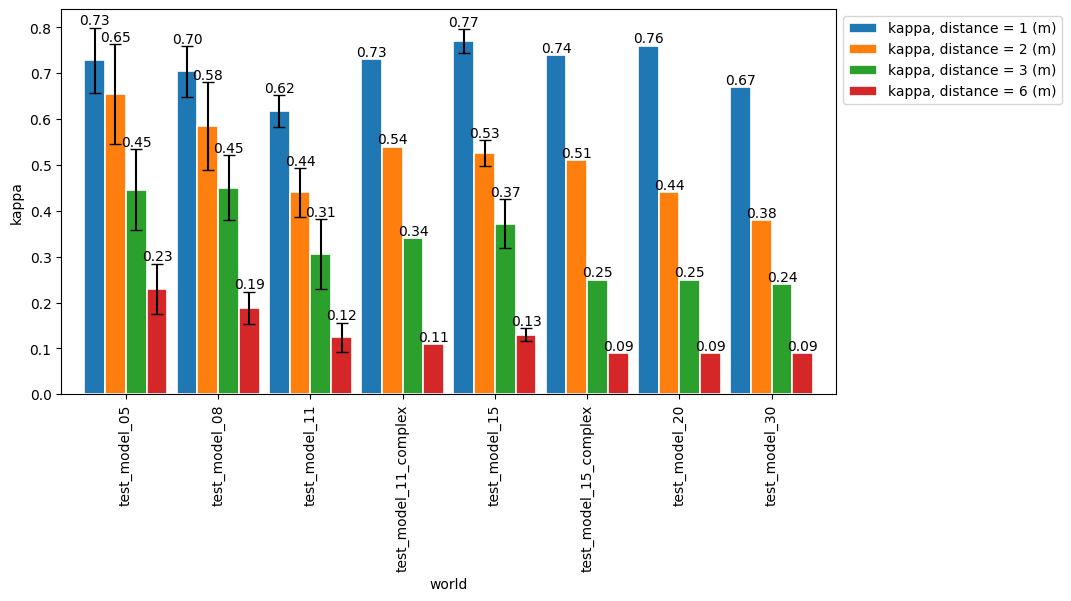
\includegraphics[width=\linewidth]{graphics/peinture_au_rouleau-kappa_vs_world_for_each_d.png}
					\caption{$\kappa$ en fonction de la densité du monde}
					\label{fig:peinture_au_rouleau-kappa_vs_world}
				\end{subfigure}
				\hfill
				\begin{subfigure}[t]{0.9\linewidth}
						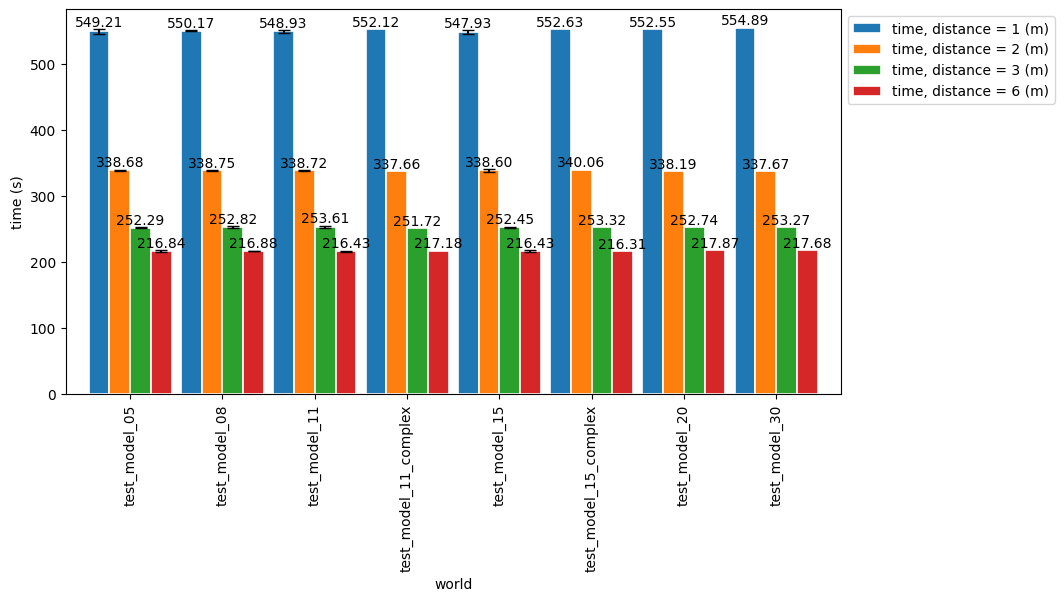
\includegraphics[width=\linewidth]{graphics/peinture_au_rouleau-time_vs_world_for_each_d.png}
						\caption{Temps d'exécution en fonction de la densité du monde}
						\label{fig:peinture_au_rouleau-time_vs_world}
				\end{subfigure}
				\caption{Évolution du score de Cohen et du temps d'exécution de l'algorithme de peinture au rouleau en fonction de la densité du monde et de la distance entre les robots.}
				\label{fig:peinture_au_rouleau-world}
			\end{figure}

			Premièrement, nous pouvons observer que le score de Cohen diminue, de manière générale, avec le nombre de zones de corrosion.
			Il existe des exceptions, notamment pour la carte composée de 15 zones de corrosion, où le score de Cohen est plus élevé que pour les cartes composées de 5, 8 et 11 zones de corrosion.
			Cela s'explique du fait que dans les cartes composées de 5, 8 et 11 zones de corrosion, nous avons introduit des zones de corrosion de formes alongées contrairement à la carte composée de 15 zones de corrosion où les zones de corrosion sont toutes des cercles.
			En effet, les zones de corrosion de formes alongées ont une probabilité plus grande de faire apparaître des zones fantômes, illustrées à la figure~\ref{fig:ghost_zone}, que les zones de corrosion de forme circulaire.
			Ces zones fantômes sont des zones libres de corrosion qui sont détectées par les crawlers.
			Il s'agit donc de faux positifs qui diminuent le score de Cohen.
			Ces zones fantômes ont également plus de chance d'apparaître lorsque la densité du monde est élevée et que donc les zones de corrosion sont plus proches les unes des autres ou encore lorsque la distance $d$ entre les deux crawlers est élevée.
			C'est bien ce que nous pouvons observer à la figure~\ref{fig:peinture_au_rouleau-kappa_vs_distance} où le score de Cohen diminue lorsque la distance $d$ entre les deux crawlers augmente.
			Nous observons qu'il semble exister une relation linéaire entre le score de Cohen et la distance $d$ entre les deux crawlers.

			\begin{figure}[h!]
				\begin{subfigure}[t]{0.49\linewidth}
					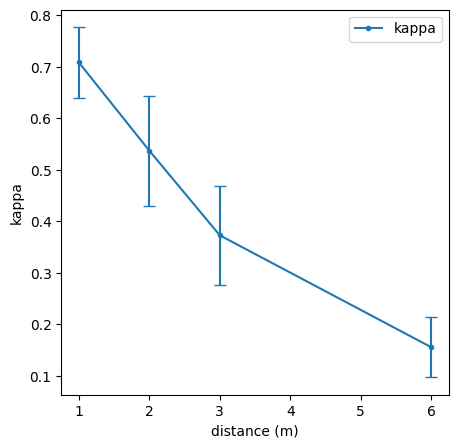
\includegraphics[width=\linewidth]{graphics/peinture_au_rouleau-kappa_vs_distance.png}
					\caption{$\kappa$ en fonction de la distance entre les deux crawlers}
					\label{fig:peinture_au_rouleau-kappa_vs_distance}
				\end{subfigure}
				\hfill
				\begin{subfigure}[t]{0.49\linewidth}
						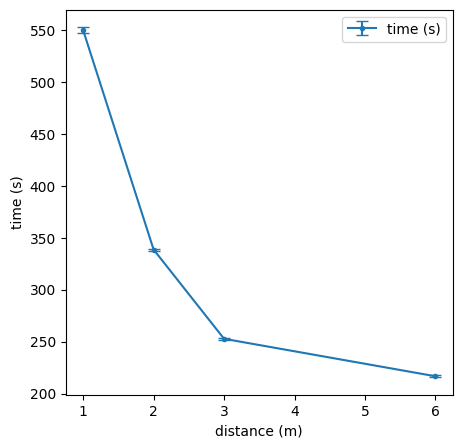
\includegraphics[width=\linewidth]{graphics/peinture_au_rouleau-time_vs_distance.png}
						\caption{Temps d'exécution en fonction de la distance entre les deux crawlers}
						\label{fig:peinture_au_rouleau-time_vs_distance}
				\end{subfigure}
				\caption{Évolution du $\kappa$ de Cohen et du temps d'exécution de l'algorithme de peinture au rouleau en fonction de la distance qui sépare les deux crawlers.}
				\label{fig:peinture_au_rouleau-distance}
			\end{figure}

			Ensuite, nous observons que le temps d'exécution de l'algorithme \textit{peinture au rouleau} est constant pour chaque valeur du nombre de zones de corrosion.
			Cela était attendu du fait que l'algorithme en question est un algorithme a priori et ne dépend donc pas du nombre de zones de corrosion.
			En revanche le temps d'exécution dépend de la distance $d$ entre les deux crawlers.
			Comme nous pouvons observer à la figure~\ref{fig:peinture_au_rouleau-time_vs_distance}, le temps d'exécution augmente lorsque la distance $d$ entre les deux crawlers diminue.
			Cela s'explique du fait que plus la distance $d$ est grande, moins les crawlers doivent effectuer de déplacements pour couvrir la carte.
			Il semble également exister une relation linéaire entre le temps d'exécution et la distance $d$ entre les deux crawlers, excepté pour la distance $d = 6$.

			\begin{figure}[h!]
				\centering
				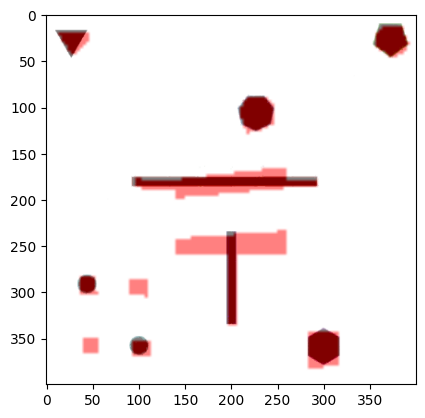
\includegraphics[width=0.5\linewidth]{graphics/output.png}
				\caption{Exemple de zone fantôme situé en bas à gauche de la carte.}
				\label{fig:ghost_zone}
			\end{figure}

			Nous avons également introduit deux cartes avec des formes plus complexes que les cartes de base.
			Malheureusement nous n'avons pas pu, par soucis de temps, faire varier la position des zones de corrosion, comme nous l'avons fait avec les cartes de faible densité.
			Néanmoins, il semble ne pas exister de différence significative entre les cartes de formes complexes et les cartes de formes simples.
			Par exemple pour les cartes avec 15 formes de corrosion et la carte avec 15 formes de corrosion complexes, le score de Cohen ne varie que de 0.02 pour une distance $d = 1$ et de 0.04 pour une distance $d = 6$.

			Dans la suite de ce rapport nous considérerons une distance $d = 3$ entre les deux crawlers pour l'algorithme \textit{peinture au rouleau}.
		\subsection*{Stratégie de navigation \textit{ski nordique}}
			Nous allons maintenant analyser les résultats obtenus pour l'algorithme \textit{ski nordique}.
			Comme pour l'algorithme \textit{peinture au rouleau}, nous avons fait varier la densité du monde et la distance $d$ entre les deux crawlers mais également le pas utilisé entre les deux crawlers.
			La figure~\ref{fig:ski_nordique-world_d} présente l'évolution du score de Cohen et du temps d'exécution de l'algorithme \textit{ski nordique} en fonction de la densité du monde pour différentes valeurs de la distance $d$ entre les deux crawlers et un pas de 3 mètres.

			\begin{figure}[h!]
				\centering
				\begin{subfigure}[t]{0.9\linewidth}
					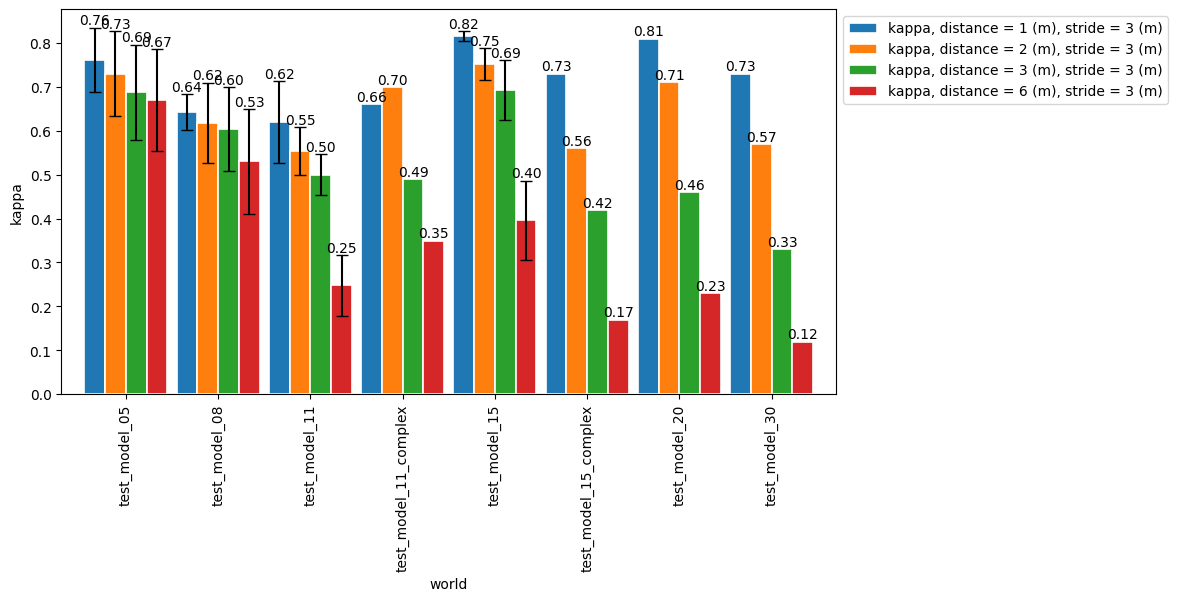
\includegraphics[width=\linewidth]{graphics/ski_nordique-kappa_vs_world_for_each_d.png}
					\caption{$\kappa$ en fonction de la densité du monde}
					\label{fig:ski_nordique-kappa_vs_world_d}
				\end{subfigure}
				\hfill
				\begin{subfigure}[t]{0.9\linewidth}
						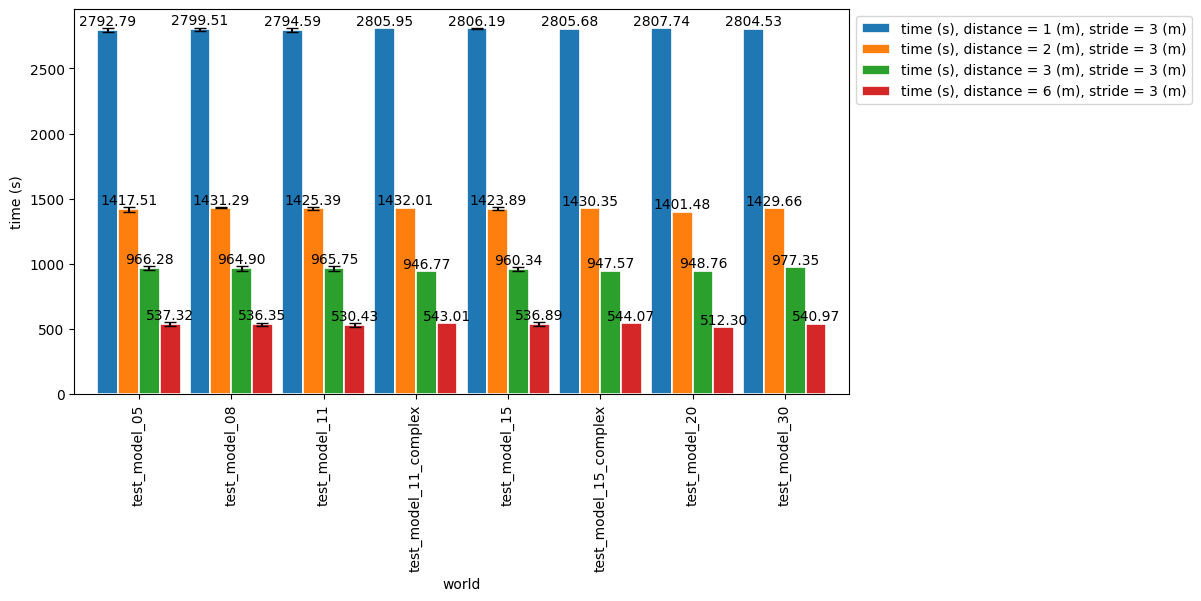
\includegraphics[width=\linewidth]{graphics/ski_nordique-time_vs_world_for_each_d.png}
						\caption{Temps d'exécution en fonction de la densité du monde}
						\label{fig:ski_nordique-time_vs_world_d}
				\end{subfigure}
				\caption{Évolution du score de Cohen et du temps d'exécution de l'algorithme de peinture au rouleau en fonction de la densité du monde pour différentes valeurs de la distance entre les deux crawlers.}
				\label{fig:ski_nordique-world_d}
			\end{figure}

			Nous avons des résultats très similaires à ceux obtenus pour l'algorithme \textit{peinture au rouleau}.
			En effet, nous observons à la figure \ref{fig:ski_nordique-kappa_vs_world_d} que le score de Cohen diminue de manière générale lorsque la densité du monde augmente.
			De plus, le temps d'exécution de l'algorithme \textit{ski nordique}, observé à la figure \ref{fig:ski_nordique-time_vs_world_d}, est constant pour chaque valeur de la densité du monde.

			\begin{figure}[h!]
				\centering
				\begin{subfigure}[t]{0.9\linewidth}
					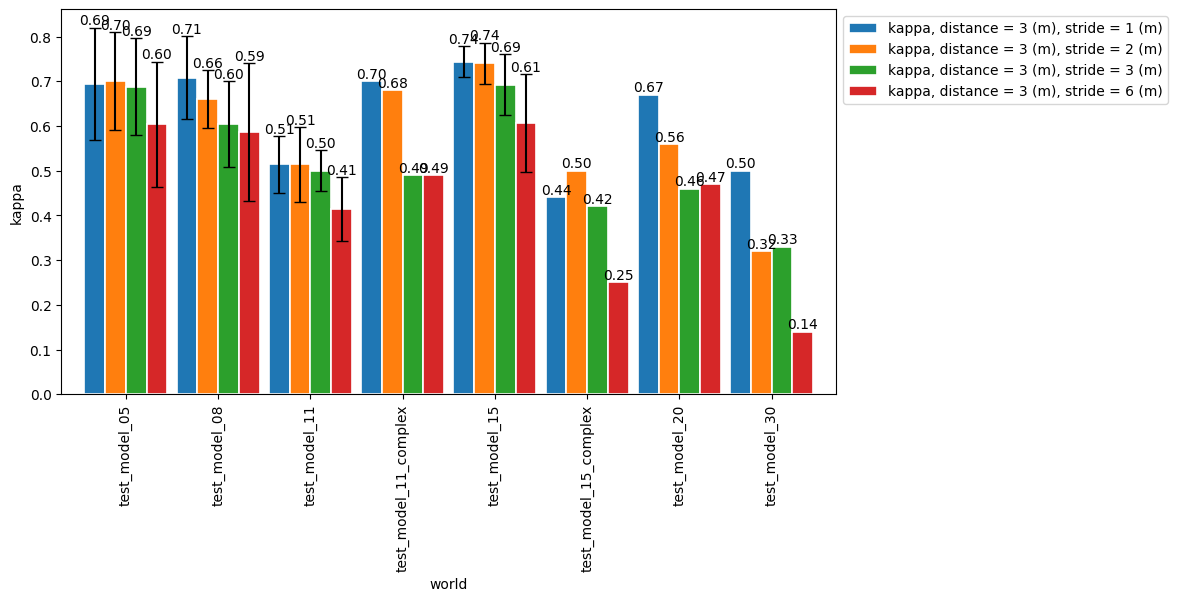
\includegraphics[width=\linewidth]{graphics/ski_nordique-kappa_vs_world_for_each_s.png}
					\caption{$\kappa$ en fonction de la densité du monde}
					\label{fig:ski_nordique-kappa_vs_world_s}
				\end{subfigure}
				\hfill
				\begin{subfigure}[t]{0.9\linewidth}
						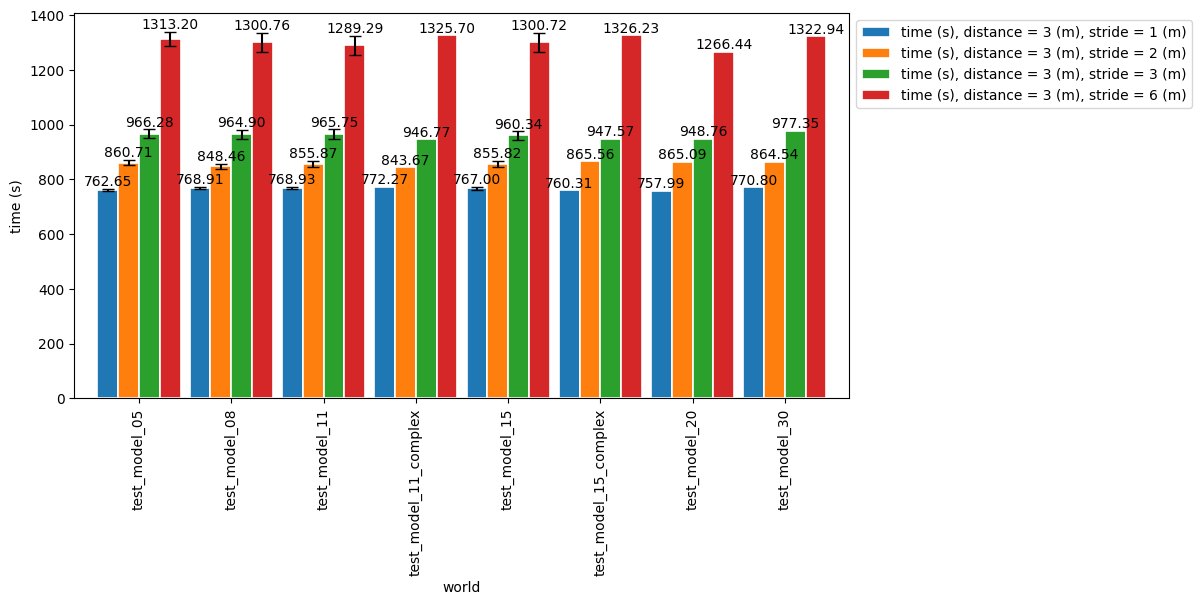
\includegraphics[width=\linewidth]{graphics/ski_nordique-time_vs_world_for_each_s.png}
						\caption{Temps d'exécution en fonction de la densité du monde}
						\label{fig:ski_nordique-time_vs_world_s}
				\end{subfigure}
				\caption{Évolution du score de Cohen et du temps d'exécution de l'algorithme de peinture au rouleau en fonction de la densité du monde pour différentes valeurs du pas entre les deux crawlers.}
				\label{fig:ski_nordique-world_s}
			\end{figure}

			Nous pouvons observer à la figure~\ref{fig:ski_nordique-world_s} l'évolution du score de Cohen et du temps d'exécution de l'algorithme \textit{ski nordique} en fonction de la densité du monde pour différentes valeurs du pas entre les deux crawlers et une distance entre les crawlers de 3 mètres.
			À la figure \ref{fig:ski_nordique-kappa_vs_world_s}, nous observons que le score de Cohen est le plus bas pour des grandes valeurs de densités et des grandes valeurs de $d$, comme pour $d = 6$ et les cartes avec 30 et 20 zones de corrosion.
			Ceci s'expplique que pour de grandes valeurs de densités et de $d$, la probabilité que les rayons du signals traversent des zones de corrosions est plus élevée.
			Il y a donc plus de chance que des zones fantômes soient créées ce qui fait diminuer le score de Cohen.
			Les formes allongées des zones de corrosion sont également un facteur qui fait diminuer le score de Cohen comme étudié précédemment.
			C'est pourquoi nous observons que le score de Cohen est le plus haut pour la carte avec la plus petite densité et sans formes allongées de corrosion, c'est-à-dire la carte avec 15 zones de corrosion.

			À la figure \ref{fig:ski_nordique-time_vs_world_s}, nous observons que le temps d'exécution de l'algorithme \textit{ski nordique} est constant pour chaque valeur de la densité du monde.
			Ceci était attendu comme pour la stratégie \textit{peinture au rouleau}.
			Cependant, nous observons que le temps d'exécution avec le pas utilisé.
			Nous nous serions plutôt attendu à ce que le temps d'exécution reste constant avec le pas des crawlers.
			En effet, indépendamment de la valeur du pas, la distance verticale et horizontale à parcourir par les crawlers est la même.
			Cette difference significative du temps d'exécution est due à la manière dont nous avons implémenté l'algorithme \textit{ski nordique} qui n'est pas optimale.
			Nous n'avons pas fait arréter les crawlers aux extrémité des plaques mais nous les avons fait continuer d'une valeur du pas en plus par simplicité d'implémentation sans penser que l'impact sur le temps d'exécution serait significatif.

			\begin{figure}[h!]
				\begin{subfigure}[t]{0.49\linewidth}
					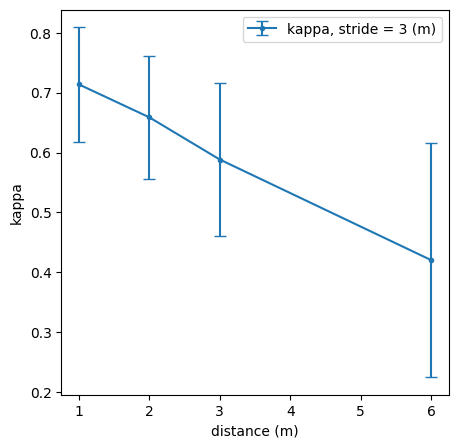
\includegraphics[width=\linewidth]{graphics/ski_nordique-kappa_vs_distance.png}
					\caption{$\kappa$ en fonction de la distance entre les deux crawlers}
					\label{fig:ski_nordique-kappa_vs_distance}
				\end{subfigure}
				\hfill
				\begin{subfigure}[t]{0.49\linewidth}
						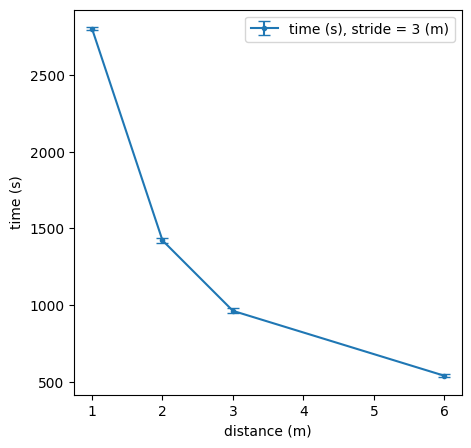
\includegraphics[width=\linewidth]{graphics/ski_nordique-time_vs_distance.png}
						\caption{Temps d'exécution en fonction de la distance entre les deux crawlers}
						\label{fig:ski_nordique-time_vs_distance}
				\end{subfigure}
				\caption{Évolution du $\kappa$ de Cohen et du temps d'exécution de l'algorithme \textit{ski nordique} en fonction de la distance qui sépare les deux crawlers.}
				\label{fig:ski_nordique-distance}
			\end{figure}

			À la figure \ref{fig:ski_nordique-distance}, nous observons l'évolution du score de Cohen et du temps d'exécution de l'algorithme \textit{ski nordique} en fonction de la distance qui sépare les deux crawlers pour un pas de 3 mètres.
			Le score semble comme pour la stratégie \textit{peinture au rouleau} suivre une relation lineaire avec la distance qui sépare les deux crawlers.
			Le temps d'exécution semble également suivre une relation linéaire avec la distance qui sépare les deux crawlers.
			Le fait que la courbe à figure \ref{fig:ski_nordique-time_vs_distance} ne soit pas une droite est dû au fait que plus la distance entre les crawlers est petite et plus le nombre de rotation que les crawlers doivent effectuer est grand.
			Or le temps de rotation n'est pas négligeable dans les temps d'exécution des algorithmes.

			\begin{figure}[h!]
				\begin{subfigure}[t]{0.49\linewidth}
					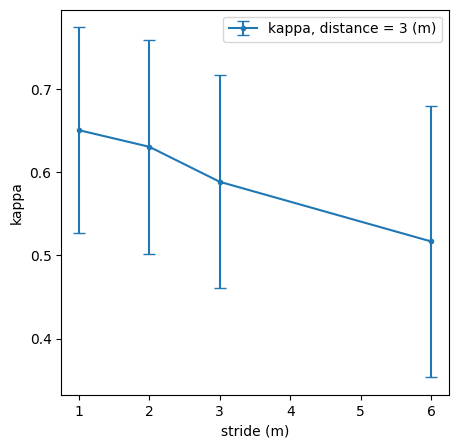
\includegraphics[width=\linewidth]{graphics/ski_nordique-kappa_vs_stride.png}
					\caption{$\kappa$ en fonction du pas des crawlers}
					\label{fig:ski_nordique-kappa_vs_stride}
				\end{subfigure}
				\hfill
				\begin{subfigure}[t]{0.49\linewidth}
						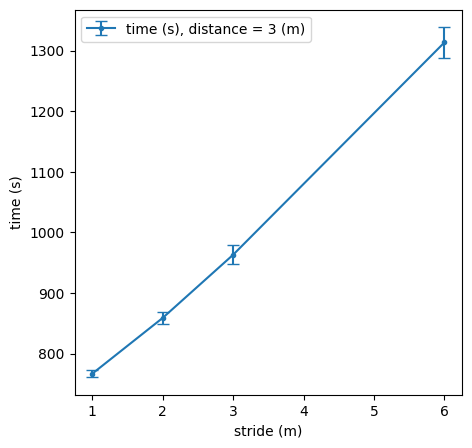
\includegraphics[width=\linewidth]{graphics/ski_nordique-time_vs_stride.png}
						\caption{Temps d'exécution en fonction du pas des crawlers}
						\label{fig:ski_nordique-time_vs_stride}
				\end{subfigure}
				\caption{Évolution du $\kappa$ de Cohen et du temps d'exécution de l'algorithme \textit{ski nordique} en fonction du pas des crawlers.}
				\label{fig:ski_nordique-stride}
			\end{figure}

			À la figure \ref{fig:ski_nordique-stride}, nous observons l'évolution du score de Cohen et du temps d'exécution de l'algorithme \textit{ski nordique} en fonction du pas des crawlers pour une distance de 3 mètres.
			Le score semble suivre une relation linéaire avec le pas des crawlers.
			Plus le pas est grand et plus le score est grand.
			Cela entre en concordance avec ce que nous expliquions précédemment.
			Plus le pas est grand et plus il y a de chance de créer des zones fantômes et donc de faire diminuer le score de Cohen.
			Le temps d'exécution lui semble suivre une relation linéaire avec le pas des crawlers.
			Comme expliqué précédemment, ce dernier aurait dû être linéaire mais notre implémentation fait dépendre le temps d'exécution du pas des crawlers.

			Ici encore il semble que le score et le temps ne soient pas affectés par le fait que les formes soient convexes ou non.

			Dans la suite de ce rapport nous considérerons une distance $d = 3$ entre les deux crawlers et un pas $s = 3$ pour l'algorithme \textit{ski nordique}.
		\subsection*{Stratégie de navigation \textit{investigation polygonale}}
			\TODO{Analyse}
		\subsection*{Comparaisons et discussions}
	\section{Bilan personnel}
		\TODO{Bilan personnel}
	\section{Conclusion et perspectives}
		\TODO{Conclusion et perspectives}
	\section*{}
	\bibliographystyle{unsrt}
	\bibliography{rapportPFE}
	\appendix
	% \section{Données collectées}
	% \section{Éléments majeurs de la conception}
	% \section{Preuves}
	\section{Implémentations techniques}
		\label{annexe:implementations}
		\subsection{Implémentation de l'algorithme \textit{peinture au rouleau}}
			\begin{lstlisting}[language=Python,caption={Implémentation de l'algorithme de peinture au rouleau},label=lst:peinture_au_rouleau]
#!/usr/bin/env python3
import rospy
import numpy
from math import *
from task_manager_lib.TaskClient import *

rospy.init_node('task_client')
server_node = rospy.get_param("~server", "/crawler_id/task_server")
default_period = rospy.get_param("~period", 0.05)
tc = TaskClient(server_node, default_period)
rospy.loginfo("Mission connected to server: " + server_node)
vel = rospy.get_param("~velocity", 0.5)
crawler_id = rospy.get_param("~crawler_id", 0)
crawlers_distance = rospy.get_param("~crawlers_distance", 1.0)
overlap = rospy.get_param("~overlap", 0.1)
width = rospy.get_param("~width", 20.0)
height = rospy.get_param("~height", 20.0)

d = crawlers_distance
k = 0
stat = 0

start = rospy.Time.now()

try:
	tc.SetStatusSync(status=stat)
	if crawler_id == 0:
		tc.WaitForStatusSync(partner="crawler_1", status=stat)
	elif crawler_id == 1:
		tc.WaitForStatusSync(partner="crawler_0", status=stat)
	stat += 1

	# vertical
	if crawler_id == 0:
		for i in numpy.arange(-width/2, width/2-d+1, d):
			tc.AlignWithTarget(goal_x=i-overlap, goal_y=height/2*(-1)**k)
			tc.FollowLine(goal_x=i-overlap, goal_y=height/2*(-1)**k, max_velocity=vel)
			tc.AlignWithTarget(goal_x=i+d-overlap, goal_y=height/2*(-1)**k)
			tc.FollowLine(goal_x=i+d-overlap, goal_y=height/2*(-1)**k, max_velocity=vel)
			k = (k+1) % 2
			tc.SetStatusSync(status=stat)
			tc.WaitForStatusSync(partner="crawler_1", status=stat)
			stat += 1
	elif crawler_id == 1:
		for i in numpy.arange(-width/2+d, width/2+1, d):
			tc.AlignWithTarget(goal_x=i+overlap, goal_y=height/2*(-1)**k)
			tc.FollowLine(goal_x=i+overlap, goal_y=height/2*(-1)**k, max_velocity=vel)
			tc.AlignWithTarget(goal_x=i+d+overlap, goal_y=height/2*(-1)**k)
			tc.FollowLine(goal_x=i+d+overlap, goal_y=height/2*(-1)**k, max_velocity=vel)
			k = (k+1) % 2
			tc.SetStatusSync(status=stat)
			tc.WaitForStatusSync(partner="crawler_0", status=stat)
			stat += 1

	if crawler_id == 0:
		tc.GoTo(goal_x=width/2+d, goal_y=-height/2, max_velocity=vel)
		tc.SetStatusSync(status=stat)
		tc.WaitForStatusSync(partner="crawler_1", status=stat)
		stat += 1
		tc.GoTo(goal_x=width/2, goal_y=-height/2, max_velocity=vel)
		tc.SetStatusSync(status=stat)
		tc.WaitForStatusSync(partner="crawler_1", status=stat)
	elif crawler_id == 1:
		tc.GoTo(goal_x=width/2+d, goal_y=-height/2+d, max_velocity=vel)
		tc.SetStatusSync(status=stat)
		tc.WaitForStatusSync(partner="crawler_0", status=stat)
		stat += 1
		tc.GoTo(goal_x=width/2, goal_y=-height/2+d, max_velocity=vel)
		tc.SetStatusSync(status=stat)
		tc.WaitForStatusSync(partner="crawler_0", status=stat)
	stat += 1
	k = 1

	# horizontal
	if crawler_id == 0:
		for i in numpy.arange(-height/2, height/2-d+1, d):
			tc.AlignWithTarget(goal_x=width/2*(-1)**k, goal_y=i-overlap)
			tc.FollowLine(goal_x=width/2*(-1)**k, goal_y=i-overlap, max_velocity=vel)
			tc.AlignWithTarget(goal_x=width/2*(-1)**k, goal_y=i+d-overlap)
			tc.FollowLine(goal_x=width/2*(-1)**k, goal_y=i+d-overlap, max_velocity=vel)
			k = (k+1) % 2
			tc.SetStatusSync(status=stat)
			tc.WaitForStatusSync(partner="crawler_1", status=stat)
			stat += 1
	elif crawler_id == 1:
		for i in numpy.arange(-height/2+d, height/2+1, d):
			tc.AlignWithTarget(goal_x=width/2*(-1)**k, goal_y=i+overlap)
			tc.FollowLine(goal_x=width/2*(-1)**k, goal_y=i+overlap, max_velocity=vel)
			tc.AlignWithTarget(goal_x=width/2*(-1)**k, goal_y=i+d+overlap)
			tc.FollowLine(goal_x=width/2*(-1)**k, goal_y=i+d+overlap, max_velocity=vel)
			k = (k+1) % 2
			tc.SetStatusSync(status=stat)
			tc.WaitForStatusSync(partner="crawler_0", status=stat)
			stat += 1

except TaskException as e:
	rospy.logerr("Exception caught: " + str(e))

end = rospy.Time.now()
time = (end-start).to_sec()
rospy.loginfo("Mission completed in " + str(time) + " seconds")
			\end{lstlisting}
		\subsection{Implémentation de l'algorithme \textit{ski nordique}}
			\begin{lstlisting}[language=Python,caption={Implémentation de l'algorithme de ski nordique},label=lst:ski_nordique]
#!/usr/bin/env python3
from time import sleep
import rospy
import numpy
from math import *
from task_manager_lib.TaskClient import *

rospy.init_node('task_client')
server_node = rospy.get_param("~server", "/crawler_id/task_server")
default_period = rospy.get_param("~period", 0.05)
tc = TaskClient(server_node, default_period)
rospy.loginfo("Mission connected to server: " + server_node)
vel = rospy.get_param("~velocity", 0.5)
crawler_id = rospy.get_param("~crawler_id", 0)
crawlers_distance = rospy.get_param("~crawlers_distance", 1.0)
stride_size = int(rospy.get_param("~stride_size", 1.0))
overlap = rospy.get_param("~overlap", 0.1)
grid_width = rospy.get_param("~grid_width", 6) // 2
grid_height = rospy.get_param("~grid_height", 6) // 2

d = crawlers_distance
k = 0
if crawler_id == 0: overlap = -overlap

start = rospy.Time.now()

# vertical pass

if crawler_id == 0: begin_w, end_w = -grid_width, grid_width + 1 - d
elif crawler_id == 1: begin_w, end_w = -grid_width + d, grid_width + 1

stat = 0
tc.SetStatusSync(status=stat)
if crawler_id == 0: tc.WaitForStatusSync(partner="crawler_1", status=stat+1)

for i in numpy.arange(begin_w, end_w, d):

	if crawler_id == 0: begin_h, end_h = -grid_height + 2*stride_size, grid_height + 1 + stride_size
	elif crawler_id == 1: begin_h, end_h = -grid_height + stride_size, grid_height + 1 + stride_size

	for j in numpy.arange(begin_h, end_h, 2*stride_size):
		tc.GoTo(goal_x=i+overlap, goal_y=j, max_velocity=vel, relative=False)
		stat += 1
		tc.SetStatusSync(status=stat)
		if crawler_id == 0: tc.WaitForStatusSync(partner="crawler_1", status=stat+1)
		elif crawler_id == 1: tc.WaitForStatusSync(partner="crawler_0", status=stat)

	tc.SetStatusSync(status=stat+1)
	if stride_size % 2 == 1:
		if crawler_id == 0: tc.GoTo(goal_x=i+overlap, goal_y=grid_height + stride_size, max_velocity=vel, relative=False)
		if crawler_id == 1: tc.GoTo(goal_x=i+overlap, goal_y=grid_height, max_velocity=vel, relative=False)
	elif stride_size % 2 == 0:
		if crawler_id == 0: tc.GoTo(goal_x=i+overlap, goal_y=grid_height, max_velocity=vel, relative=False)
		if crawler_id == 1: tc.GoTo(goal_x=i+overlap, goal_y=grid_height + stride_size, max_velocity=vel, relative=False)
	stat = 0
	tc.SetStatusSync(status=stat)
	if crawler_id == 1 and stride_size % 2 == 1: tc.WaitForStatusSync(partner="crawler_0", status=stat+1)
	elif crawler_id == 0 and stride_size % 2 == 0: tc.WaitForStatusSync(partner="crawler_1", status=stat+1)

	if stride_size % 2 == 1:
		if crawler_id == 0: begin_h, end_h = grid_height - stride_size, -grid_height - 1 - stride_size
		elif crawler_id == 1: begin_h, end_h = grid_height - 2*stride_size, -grid_height - 1 - stride_size
	elif stride_size % 2 == 0:
		if crawler_id == 0: begin_h, end_h = grid_height - 2*stride_size, -grid_height - 1 - stride_size
		elif crawler_id == 1: begin_h, end_h = grid_height - stride_size, -grid_height - 1 - stride_size

	for j in numpy.arange(begin_h, end_h, -2*stride_size):
		tc.GoTo(goal_x=i+overlap, goal_y=j, max_velocity=vel, relative=False)
		stat += 1
		tc.SetStatusSync(status=stat)
		if crawler_id == 0 and stride_size % 2 == 1: tc.WaitForStatusSync(partner="crawler_1", status=stat)
		if crawler_id == 0 and stride_size % 2 == 0: tc.WaitForStatusSync(partner="crawler_1", status=stat+1)
		elif crawler_id == 1 and stride_size % 2 == 1: tc.WaitForStatusSync(partner="crawler_0", status=stat+1)
		elif crawler_id == 1 and stride_size % 2 == 0: tc.WaitForStatusSync(partner="crawler_0", status=stat)

	tc.SetStatusSync(status=stat+1)
	if crawler_id == 0: tc.GoTo(goal_x=i+d+overlap, goal_y=-grid_height, max_velocity=vel, relative=False)
	if crawler_id == 1: tc.GoTo(goal_x=i+d+overlap, goal_y=-grid_height - stride_size, max_velocity=vel, relative=False)
	stat = 0
	tc.SetStatusSync(status=stat)
	if crawler_id == 0: tc.WaitForStatusSync(partner="crawler_1", status=stat+1)

tc.SetStatusSync(status=stat+1)

# repostioning

stat = 0
tc.SetStatusSync(status=stat)

if crawler_id == 0: tc.GoTo(goal_x=grid_width, goal_y=-grid_height, max_velocity=vel, relative=False)
elif crawler_id == 1: tc.GoTo(goal_x=grid_width + stride_size, goal_y=-grid_height + d, max_velocity=vel, relative=False)

if crawler_id == 0: tc.WaitForStatusSync(partner="crawler_1", status=stat+1)

# horizontal pass

if crawler_id == 0: begin_h, end_h = -grid_height, grid_height + 1 - d
elif crawler_id == 1: begin_h, end_h = -grid_height + d, grid_height + 1

# stat = 0
# tc.SetStatusSync(status=stat)
# if crawler_id == 0: tc.WaitForStatusSync(partner="crawler_1", status=stat+1)

for j in numpy.arange(begin_h, end_h, d):

	if crawler_id == 0: begin_w, end_w = grid_width - 2*stride_size, -grid_width - 1 - stride_size
	elif crawler_id == 1: begin_w, end_w = grid_width - stride_size, -grid_width - 1 - stride_size

	for i in numpy.arange(begin_w, end_w, -2*stride_size):
		tc.GoTo(goal_x=i, goal_y=j+overlap, max_velocity=vel, relative=False)
		stat += 1
		tc.SetStatusSync(status=stat)
		if crawler_id == 0: tc.WaitForStatusSync(partner="crawler_1", status=stat+1)
		elif crawler_id == 1: tc.WaitForStatusSync(partner="crawler_0", status=stat)

	tc.SetStatusSync(status=stat+1)
	if stride_size % 2 == 1:
		if crawler_id == 0: tc.GoTo(goal_x=-grid_width - stride_size, goal_y=j+overlap, max_velocity=vel, relative=False)
		if crawler_id == 1: tc.GoTo(goal_x=-grid_width, goal_y=j+overlap, max_velocity=vel, relative=False)
	elif stride_size % 2 == 0:
		if crawler_id == 0: tc.GoTo(goal_x=-grid_width, goal_y=j+overlap, max_velocity=vel, relative=False)
		if crawler_id == 1: tc.GoTo(goal_x=-grid_width - stride_size, goal_y=j+overlap, max_velocity=vel, relative=False)
	stat = 0
	tc.SetStatusSync(status=stat)
	if crawler_id == 1 and stride_size % 2 == 1: tc.WaitForStatusSync(partner="crawler_0", status=stat+1)
	if crawler_id == 0 and stride_size % 2 == 0: tc.WaitForStatusSync(partner="crawler_1", status=stat+1)

	if stride_size % 2 == 1:
		if crawler_id == 0: begin_w, end_w = -grid_width + stride_size, grid_width + 1 + stride_size
		elif crawler_id == 1: begin_w, end_w = -grid_width + 2*stride_size, grid_width + 1 + stride_size
	elif stride_size % 2 == 0:
		if crawler_id == 0: begin_w, end_w = -grid_width + 2*stride_size, grid_width + 1 + stride_size
		elif crawler_id == 1: begin_w, end_w = -grid_width + stride_size, grid_width + 1 + stride_size

	for i in numpy.arange(begin_w, end_w, 2*stride_size):
		tc.GoTo(goal_x=i, goal_y=j+overlap, max_velocity=vel, relative=False)
		stat += 1
		tc.SetStatusSync(status=stat)
		if crawler_id == 0 and stride_size % 2 == 1: tc.WaitForStatusSync(partner="crawler_1", status=stat)
		if crawler_id == 0 and stride_size % 2 == 0: tc.WaitForStatusSync(partner="crawler_1", status=stat+1)
		elif crawler_id == 1 and stride_size % 2 == 1: tc.WaitForStatusSync(partner="crawler_0", status=stat+1)
		elif crawler_id == 1 and stride_size % 2 == 0: tc.WaitForStatusSync(partner="crawler_0", status=stat)

	if crawler_id == 1: tc.SetStatusSync(status=stat+1)
	if crawler_id == 0: tc.GoTo(goal_x=grid_width, goal_y=j+d+overlap, max_velocity=vel, relative=False)
	if crawler_id == 1: tc.GoTo(goal_x=grid_width + stride_size, goal_y=j+d+overlap, max_velocity=vel, relative=False)
	stat = 0
	tc.SetStatusSync(status=stat)
	if crawler_id == 0: tc.WaitForStatusSync(partner="crawler_1", status=stat+1)

tc.SetStatusSync(status=stat+1)

end = rospy.Time.now()
time = (end-start).to_sec()
rospy.loginfo("Mission completed in " + str(time) + " seconds")

			\end{lstlisting}
		\subsection{Implémentation de l'algorithme \textit{investigation polygonale}}
			\begin{lstlisting}[language=Python,caption={Implémentation de l'algorithme d'investigation polygonale},label=lst:investigation_polygonale]
#!/usr/bin/env python3
# ROS specific imports
import roslib; roslib.load_manifest('floor_nav')
import rospy
import os
import tf
from task_manager_lib.TaskClient import *
from nav_msgs.msg import OccupancyGrid
from visualization_msgs.msg import MarkerArray
from visualization_msgs.msg import Marker
from geometry_msgs.msg import Point
from CrawlerOccupancyGrid import *
import numpy as np
from oct2py import octave
from math import sqrt
from time import sleep

DEFAULT_UWB_POWER_RX_THRESHOLD = 0
DEFAULT_N_CRAWLERS = 2
DEFAULT_N_POINTS = 4
DEFAULT_SCALE = 10
DEFAULT_DELTA = 5.0

def mission(centroids_map, polygons_map, radii_map, crawler_id, n_crawlers, n_points, cruise_velocity, investigation_velocity, idx=None, tm=None):
	print("Starting mission")
	start = rospy.Time.now()

	print(f'Number of crawlers: {n_crawlers}')

	if n_crawlers == 2:
		for centroid in range(len(centroids_map)):
			if idx is not None and centroid < idx: continue

			print(f'Investigating centroid {centroid}')

			file = open("/home/chroma/Downloads/mission.txt", "w")
			file.write(f'{centroid}\n')
			end = rospy.Time.now()
			if tm is not None: time = (end-start).to_sec() + tm
			else: time = (end-start).to_sec()
			file.write(f'{time}\n')
			file.close()
			os.system("rosservice call /save_occgrid")

			tc.AlignWithTarget(goal_x=polygons_map[centroid][crawler_id][0], goal_y=polygons_map[centroid][crawler_id][1], angle_threshold=0.05)
			tc.FollowLine(goal_x=polygons_map[centroid][crawler_id][0], goal_y=polygons_map[centroid][crawler_id][1], max_velocity=cruise_velocity)

			first_turn = True

			stat = 0
			tc.SetStatusSync(status=stat)
			if crawler_id == 0: tc.WaitForStatusSync(partner="crawler_1", status=stat)
			elif crawler_id == 1: tc.WaitForStatusSync(partner="crawler_0", status=stat)

			crawler_position = crawler_id
			polygon = polygons_map[centroid]
			radii = radii_map[centroid]

			area_x = radii[0] - 0.1
			area_w = radii[2] + 0.3
			area_y = radii[1] - 0.1
			area_h = radii[3] + 0.3

			stat = 0
			tc.SetStatusSync(status=stat)
			if crawler_id == 1: tc.WaitForStatusSync(partner="crawler_0", status=stat+1)

			for _ in range(0, n_points, n_crawlers):
				w4Completion = tc.WaitForCompletion(x=area_x, y=area_y, w=area_w, h=area_h, foreground=False)
				tc.addCondition(ConditionIsCompleted("Completion detector", tc, w4Completion))
				try:
					for _ in range(1, n_points - n_crawlers + 1):
						crawler_position = (crawler_position - 1) % n_points
						tc.AlignWithTarget(goal_x=polygon[crawler_position][0], goal_y=polygon[crawler_position][1])
						tc.FollowLine(goal_x=polygon[crawler_position][0], goal_y=polygon[crawler_position][1], max_velocity=investigation_velocity)
					first_turn = False
				except TaskConditionException as e:
					rospy.loginfo("Path following interrupted on condition: %s" % " or ".join([str(c) for c in e.conditions]))
				except TaskException as e:
					print(e)

				tc.clearConditions()
				tc.stopTask(w4Completion)

				stat += 1
				tc.SetStatusSync(status=stat)
				if crawler_id == 0 and not first_turn: tc.WaitForStatusSync(partner="crawler_1", status=stat)
				elif crawler_id == 1 and not first_turn and stat < n_points: tc.WaitForStatusSync(partner="crawler_0", status=stat+1)
				# if crawler_id == 0: tc.WaitForStatusSync(partner="crawler_1", status=stat)
				# elif crawler_id == 1 and stat < n_points: tc.WaitForStatusSync(partner="crawler_0", status=stat+1)

			tc.SetStatusSync(status=stat+1)
			tc.clearConditions()
			tc.stopTask(w4Completion)
	elif n_crawlers == 3:
		for centroid in range(len(centroids_map)):
			if idx is not None and centroid < idx: continue

			print(f'Investigating centroid {centroid}')

			file = open("/home/chroma/Downloads/mission.txt", "w")
			file.write(f'{centroid}\n')
			end = rospy.Time.now()
			if tm is not None: time = (end-start).to_sec() + tm
			else: time = (end-start).to_sec()
			file.write(f'{time}\n')
			file.close()
			os.system("rosservice call /save_occgrid")

			tc.AlignWithTarget(goal_x=polygons_map[centroid][crawler_id][0], goal_y=polygons_map[centroid][crawler_id][1], angle_threshold=0.05)
			tc.FollowLine(goal_x=polygons_map[centroid][crawler_id][0], goal_y=polygons_map[centroid][crawler_id][1], max_velocity=cruise_velocity)

			stat = 0
			tc.SetStatusSync(status=stat)
			if crawler_id == 0: tc.WaitForStatusSync(partner="crawler_1", status=stat)
			if crawler_id == 0: tc.WaitForStatusSync(partner="crawler_2", status=stat)
			if crawler_id == 1: tc.WaitForStatusSync(partner="crawler_0", status=stat)
			if crawler_id == 1: tc.WaitForStatusSync(partner="crawler_2", status=stat)
			if crawler_id == 2: tc.WaitForStatusSync(partner="crawler_0", status=stat)
			if crawler_id == 2: tc.WaitForStatusSync(partner="crawler_1", status=stat)

			print(f'Ready crawler {crawler_id}')

			crawler_position = crawler_id
			polygon = polygons_map[centroid]
			radii = radii_map[centroid]

			area_x = radii[0] - 0.1
			area_w = radii[2] + 0.3
			area_y = radii[1] - 0.1
			area_h = radii[3] + 0.3

			stat = 0
			tc.SetStatusSync(status=stat)
			if crawler_id == 1: tc.WaitForStatusSync(partner="crawler_0", status=stat+1)
			elif crawler_id == 2: tc.WaitForStatusSync(partner="crawler_1", status=stat+1)

			for _ in range(0, n_points, n_crawlers + crawler_id):
				w4Completion = tc.WaitForCompletion(x=area_x, y=area_y, w=area_w, h=area_h, foreground=False)
				tc.addCondition(ConditionIsCompleted("Completion detector", tc, w4Completion))
				try:
					for _ in range(0, n_points - n_crawlers):
						crawler_position = (crawler_position - 1) % n_points
						tc.AlignWithTarget(goal_x=polygon[crawler_position][0], goal_y=polygon[crawler_position][1])
						tc.FollowLine(goal_x=polygon[crawler_position][0], goal_y=polygon[crawler_position][1], max_velocity=investigation_velocity)
				except TaskConditionException as e:
					rospy.loginfo("Path following interrupted on condition: %s" % " or ".join([str(c) for c in e.conditions]))
				except TaskException as e:
					print(e)

				tc.clearConditions()
				tc.stopTask(w4Completion)

				stat += 1
				tc.SetStatusSync(status=stat)
				if crawler_id == 0 and stat < 2: tc.WaitForStatusSync(partner="crawler_2", status=stat)
				elif crawler_id == 1: tc.WaitForStatusSync(partner="crawler_0", status=stat+1)
				elif crawler_id == 2: tc.WaitForStatusSync(partner="crawler_1", status=stat+1)

			if crawler_id == 1 and stat == 1: tc.SetStatusSync(status=stat+1)
			if crawler_id == 2 and stat == 1:
				tc.AlignWithTarget(goal_x=polygons_map[centroid][1][0] - 0.5, goal_y=polygons_map[centroid][1][1] + 0.5, angle_threshold=0.05)
				tc.FollowLine(goal_x=polygons_map[centroid][1][0] - 0.5, goal_y=polygons_map[centroid][1][1] + 0.5, max_velocity=cruise_velocity)
				tc.Wait(duration=5.0)

	end = rospy.Time.now()
	if tm is not None: time = (end-start).to_sec() + tm
	else: time = (end-start).to_sec()
	rospy.loginfo("Mission completed in " + str(time) + " seconds")

	os.system("rm /home/chroma/Downloads/mission.txt")

def solve_TSP(centroids_map):
	import math
	from itertools import combinations
	import gurobipy as gp
	from gurobipy import GRB

	# Callback - use lazy constraints to eliminate sub-tours
	def subtourelim(model, where):
		if where == GRB.Callback.MIPSOL:
			vals = model.cbGetSolution(model._vars)
			# find the shortest cycle in the selected edge list
			tour = subtour(vals)
			if len(tour) < n:
				# add subtour elimination constr. for every pair of cities in tour
				model.cbLazy(gp.quicksum(model._vars[i, j] for i, j in combinations(tour, 2)) <= len(tour)-1)

	# Given a tuplelist of edges, find the shortest subtour
	def subtour(vals):
		# make a list of edges selected in the solution
		edges = gp.tuplelist((i, j) for i, j in vals.keys() if vals[i, j] > 0.5)
		unvisited = list(range(n))
		cycle = range(n+1)  # initial length has 1 more city
		while unvisited:  # true if list is non-empty
			thiscycle = []
			neighbors = unvisited
			while neighbors:
				current = neighbors[0]
				thiscycle.append(current)
				unvisited.remove(current)
				neighbors = [j for i, j in edges.select(current, '*') if j in unvisited]
			if len(cycle) > len(thiscycle):
				cycle = thiscycle
		return cycle

	n = len(centroids_map)
	points = [(centroids_map[i][0], centroids_map[i][1]) for i in range(n)]

	# Dictionary of Euclidean distance between each pair of points
	dist = {(i, j): math.sqrt(sum((points[i][k]-points[j][k])**2 for k in range(2))) for i in range(n) for j in range(i)}

	m = gp.Model()

	# Create variables
	vars = m.addVars(dist.keys(), obj=dist, vtype=GRB.BINARY, name='e')
	for i, j in vars.keys():
		vars[j, i] = vars[i, j]  # edge in opposite direction

	# Add degree-2 constraint
	m.addConstrs(vars.sum(i, '*') == 2 for i in range(n))

	# Optimize model
	m._vars = vars
	m.Params.LazyConstraints = 1
	m.optimize(subtourelim)

	vals = m.getAttr('X', vars)
	tour = subtour(vals)
	assert len(tour) == n

	print(f'Optimal tour: {tour}')
	print(f'Optimal cost: {m.objVal}')

	return tour

def solve_mTSP(centroids_map, perimeters_map, n_crawlers):
	"""
		Returns a permutation of the centroids_map that minimizes the total distance traveled by the crawlers
	"""

	def d(x1, y1, x2, y2):
		return sqrt((x1-x2)**2 + (y1-y2)**2) + 50.0

	octave.addpath('/home/chroma/Documents/Multi-robot_navigation_and_control_for_acoustic_inspection_of_metal_plate_structures/scripts/')
	octave.eval('pkg load statistics')

	XY = np.array(centroids_map)
	max_salesmen = n_crawlers
	depots = np.array([
		[-3, -4.0],
		[3.0, -4.0]
	])
	CostType = 2
	MIN_TOUR = 1
	POP_SIZE = 256
	NUM_ITER = 100
	SHOW_PROG = True
	SHOW_RES = True
	DMAT = np.zeros((len(XY), len(XY)))
	for i in range(len(XY)):
		for j in range(len(XY)):
			DMAT[i, j] = d(XY[i, 0], XY[i, 1], XY[j, 0], XY[j, 1])
	[min_dist, best_tour, generation] = octave.mdmtspv_ga(XY, max_salesmen, depots, CostType, MIN_TOUR, POP_SIZE, NUM_ITER, SHOW_PROG, SHOW_RES, DMAT, nout=3)
	print("Minimum distance: ")
	print(min_dist)
	print("Best tour: ")
	print(best_tour)
	print("Generation: ")
	print(generation)

	sleep(10000000)

if __name__ == '__main__':
	rospy.init_node('task_client')
	server_node = rospy.get_param("~server", "/crawler_id/task_server")
	default_period = rospy.get_param("~period", 0.05)
	tc = TaskClient(server_node, default_period)
	investigation_velocity = rospy.get_param("~investigation_velocity", 0.3)
	cruise_velocity = rospy.get_param("~cruise_velocity", 1.)
	uwb_power_rx_threshold = rospy.get_param("~uwb_power_rx_threshold", DEFAULT_UWB_POWER_RX_THRESHOLD)
	n_crawlers = rospy.get_param("~n_crawlers", DEFAULT_N_CRAWLERS)
	n_points = rospy.get_param("~n_points", DEFAULT_N_POINTS)
	scale = rospy.get_param("~scale", DEFAULT_SCALE)
	delta = rospy.get_param("~delta", DEFAULT_DELTA)
	crawler_id = rospy.get_param("~crawler_id", 0)
	depot_x = rospy.get_param("~depot_x", -3.0)
	depot_y = rospy.get_param("~depot_y", -3.0)
	filename = rospy.get_param("~filename", '')
	occ_grid = CrawlerOccupancyGrid(
		rospy.get_param("~grid_width", rospy.get_param("~grid_width", DEFAULT_GRID_WIDTH)),
		rospy.get_param("~grid_height", rospy.get_param("~grid_height", DEFAULT_GRID_HEIGHT)),
		rospy.get_param("~grid_resolution", rospy.get_param("~grid_resolution", DEFAULT_GRID_RESOLUTION))
	)

	listener = tf.TransformListener()

	pub_centroid = rospy.Publisher("~circle", MarkerArray, queue_size=1)
	pub_polygone = rospy.Publisher("~poly", MarkerArray, queue_size=1)
	pub_occgrid = rospy.Publisher("~occ_grid", OccupancyGrid, queue_size=1)

	occ_grid.restore_from_image(filename)

	centroids_grid, radii_grid = occ_grid.find_centroid_of_clusters()
	centroids_map = []
	radii_map = []
	for i in range(len(centroids_grid)):
		centroids_map.append((centroids_grid[i][0] * occ_grid.resolution - occ_grid.width / 2.0, centroids_grid[i][1] * occ_grid.resolution - occ_grid.height / 2.0))
		radii_map.append((radii_grid[i][0] * occ_grid.resolution - occ_grid.width / 2.0, radii_grid[i][1] * occ_grid.resolution - occ_grid.height / 2.0, radii_grid[i][2] * occ_grid.resolution, radii_grid[i][3] * occ_grid.resolution))
	polygons_grid = []
	polygons_map = []
	for i in range(len(centroids_grid)):
		vertices_grid = occ_grid.get_polygone_around_centroid(n_points, centroids_grid[i], radii_grid[i][2:4] / 2.0, scale, delta)
		vertices_map = []
		for j in range(len(vertices_grid)):
			vertices_map.append((vertices_grid[j][0] * occ_grid.resolution - occ_grid.width / 2.0, vertices_grid[j][1] * occ_grid.resolution - occ_grid.height / 2.0))
		polygons_grid.append(vertices_grid)
		polygons_map.append(vertices_map)

	perimeters_grid = []
	perimeters_map = []
	for i in range(len(centroids_grid)):
		perimeters_grid.append(occ_grid.get_perimeter_of_polygone(polygons_grid[i]))
		perimeters_map.append(occ_grid.get_perimeter_of_polygone(polygons_map[i]))

	tour = solve_TSP(centroids_map)
	depot = (depot_x, depot_y)
	# find closest centroid to depot
	min_dist = 100000
	min_index = 0
	for i in range(len(centroids_map)):
		dist = sqrt((centroids_map[i][0] - depot[0]) ** 2 + (centroids_map[i][1] - depot[1]) ** 2)
		if dist < min_dist:
			min_dist = dist
			min_index = i
	# shift tour so that the closest centroid to depot is the first one
	tour = tour[min_index:] + tour[:min_index]

	# reorder centroids, radii, polygons and perimeters according to tour
	centroids_map = [centroids_map[i] for i in tour]
	radii_map = [radii_map[i] for i in tour]
	polygons_map = [polygons_map[i] for i in tour]
	perimeters_map = [perimeters_map[i] for i in tour]

	print(f"tour: {tour}")
	print(f"centroids_map: {centroids_map}")

	if os.path.isfile("/home/chroma/Downloads/occupancy_grid.png"):
		occ_grid.restore_from_image("/home/chroma/Downloads/occupancy_grid.png")

	marker_array = MarkerArray()
	for i in range(len(centroids_map)):
		marker = Marker()
		marker.header.frame_id = "world"
		marker.header.stamp = rospy.Time.now()
		marker.ns = "circle"
		marker.id = i
		marker.type = Marker.CYLINDER
		marker.action = Marker.ADD
		marker.pose.position.x = centroids_map[i][0]
		marker.pose.position.y = centroids_map[i][1]
		marker.pose.position.z = 0.0
		marker.pose.orientation.x = 0.0
		marker.pose.orientation.y = 0.0
		marker.pose.orientation.z = 0.0
		marker.pose.orientation.w = 1.0
		marker.scale.x = 0.1
		marker.scale.y = 0.1
		marker.scale.z = 0.1
		marker.color.a = 1.0
		marker.color.r = 0.0
		marker.color.g = 1.0
		marker.color.b = 0.0
		marker_array.markers.append(marker)

	marker_array_2 = MarkerArray()
	for i in range(len(centroids_map)):
		for j in range(n_points):
			marker = Marker()
			marker.header.frame_id = "world"
			marker.header.stamp = rospy.Time.now()
			marker.ns = "poly"
			marker.id = i * n_points + j
			marker.type = Marker.LINE_STRIP
			marker.action = Marker.ADD
			marker.pose.position.x = 0.0
			marker.pose.position.y = 0.0
			marker.pose.position.z = 0.0
			marker.pose.orientation.x = 0.0
			marker.pose.orientation.y = 0.0
			marker.pose.orientation.z = 0.0
			marker.pose.orientation.w = 1.0
			marker.scale.x = 0.01
			marker.scale.y = 0.01
			marker.scale.z = 0.01
			marker.color.a = 1.0
			marker.color.r = 1.0
			marker.color.g = 0.0
			marker.color.b = 0.0
			point = Point()
			point.x = polygons_map[i][j][0]
			point.y = polygons_map[i][j][1]
			point.z = 0.0
			marker.points.append(point)
			point = Point()
			point.x = polygons_map[i][(j + 1) % n_points][0]
			point.y = polygons_map[i][(j + 1) % n_points][1]
			point.z = 0.0
			marker.points.append(point)
			marker_array_2.markers.append(marker)

	pub_centroid.publish(marker_array)
	pub_polygone.publish(marker_array_2)
	occ_grid.publish(pub_occgrid, rospy.Time.now())

	if os.path.isfile("/home/chroma/Downloads/mission.txt"):
		file = open("/home/chroma/Downloads/mission.txt", "r")
		lines = file.readlines()
		file.close()
		idx = int(lines[0])
		tm = float(lines[1])
		mission(centroids_map, polygons_map, radii_map, crawler_id, n_crawlers, n_points, cruise_velocity, investigation_velocity, idx, tm)
	else:
		mission(centroids_map, polygons_map, radii_map, crawler_id, n_crawlers, n_points, cruise_velocity, investigation_velocity)

			\end{lstlisting}
	\section{Environnements de test}
		\label{annexe:cartes}
		\begin{figure}[H]
			\centering
			\begin{subfigure}[t]{\linewidth}
				\centering
				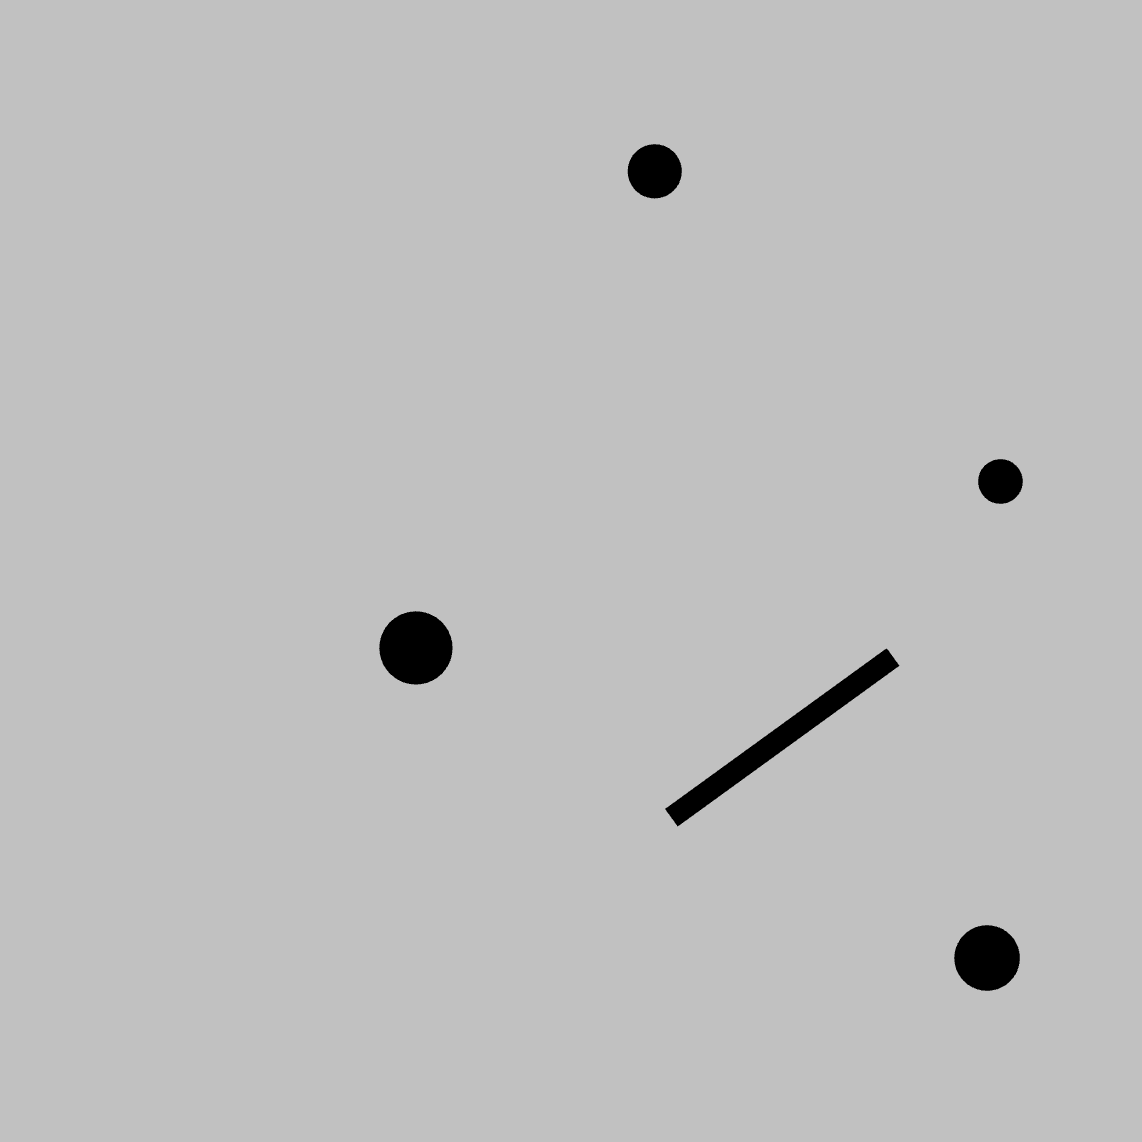
\includegraphics[width=0.15\linewidth]{graphics/test_model_05_1.png}
				\hfill
				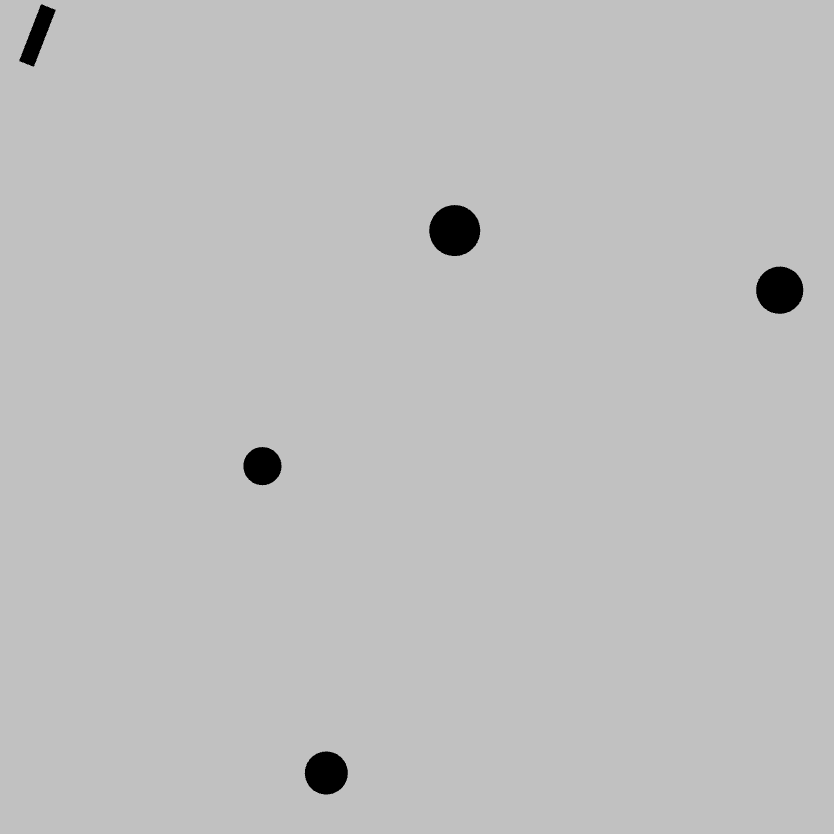
\includegraphics[width=0.15\linewidth]{graphics/test_model_05_2.png}
				\hfill
				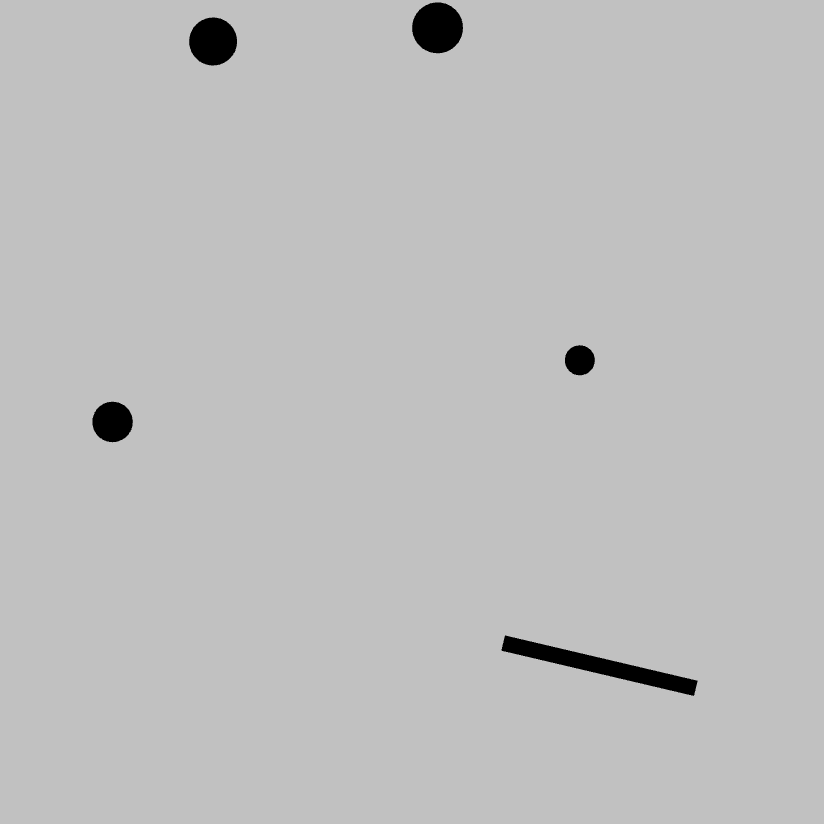
\includegraphics[width=0.15\linewidth]{graphics/test_model_05_3.png}
				\hfill
				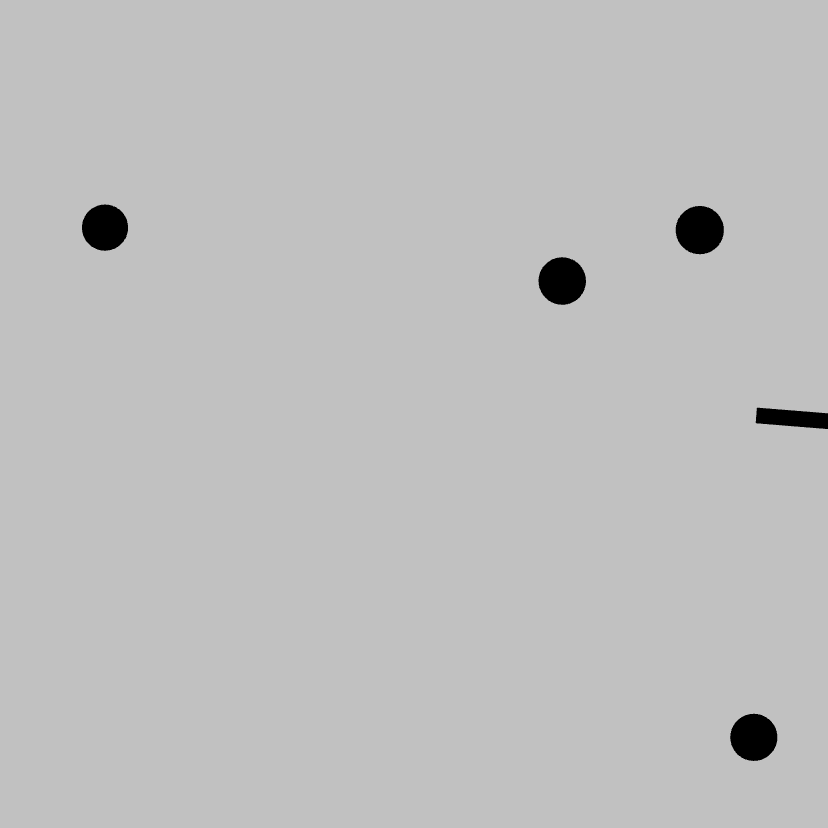
\includegraphics[width=0.15\linewidth]{graphics/test_model_05_4.png}
				\hfill
				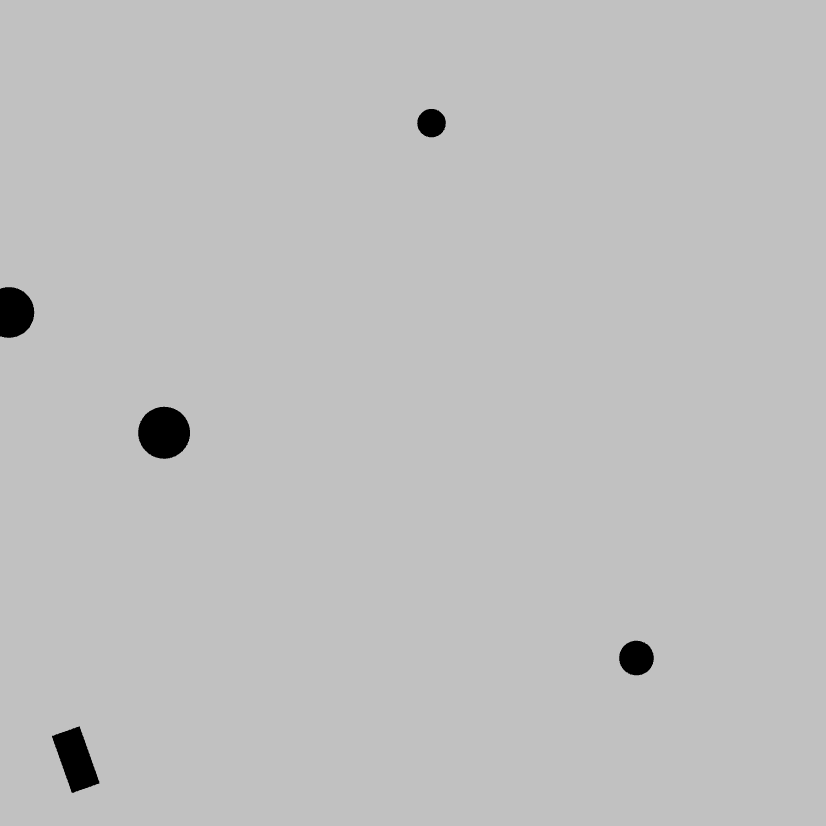
\includegraphics[width=0.15\linewidth]{graphics/test_model_05_5.png}
				\caption{Testing worlds with 5 corrosion areas}
				\label{fig:test_model_05_5}
			\end{subfigure}
			\hfill
			\begin{subfigure}[t]{\linewidth}
				\centering
				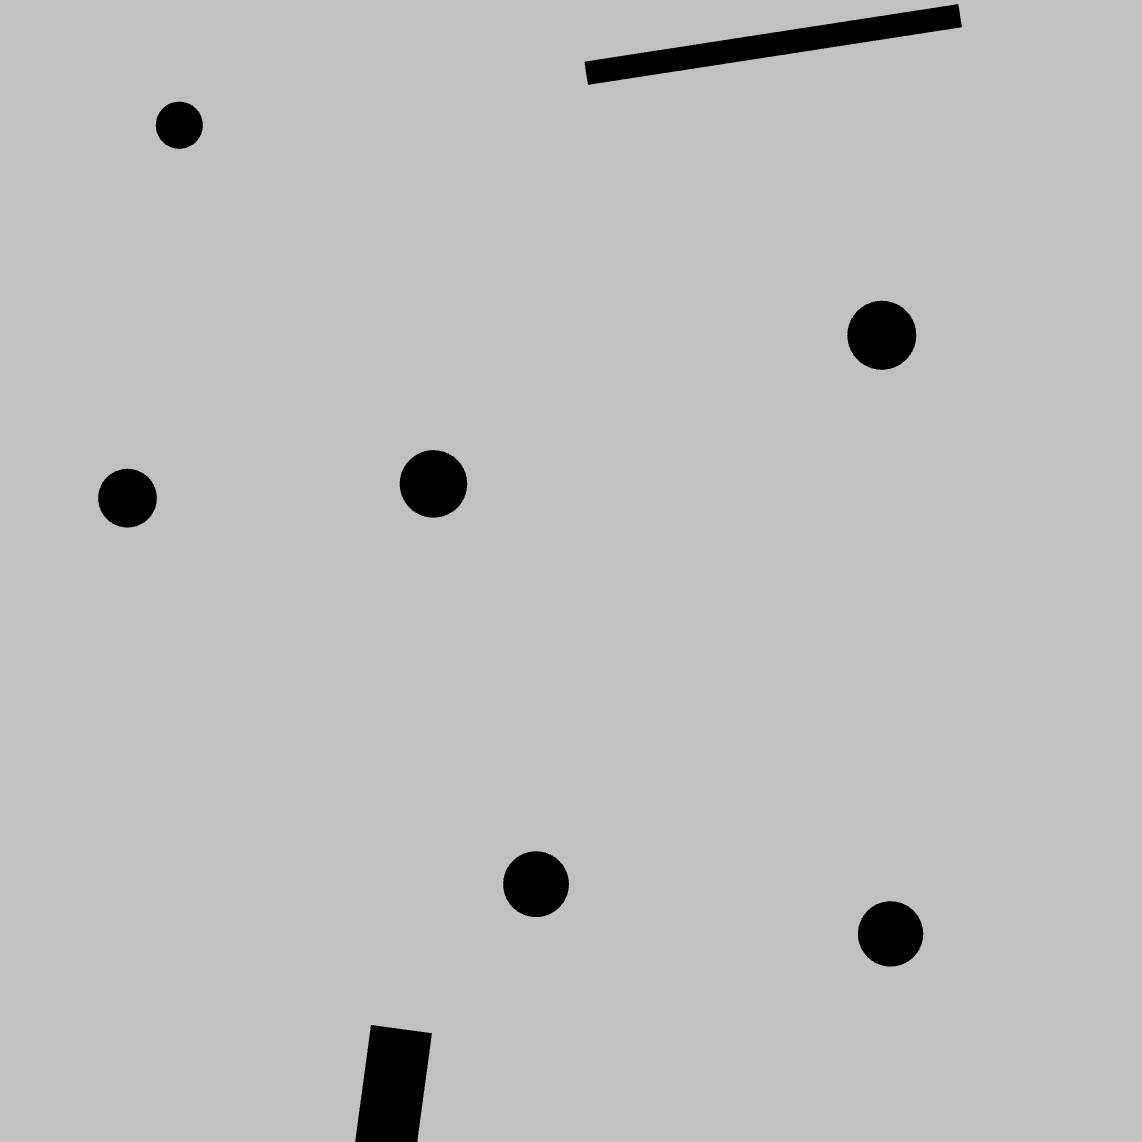
\includegraphics[width=0.15\linewidth]{graphics/test_model_08_1.png}
				\hfill
				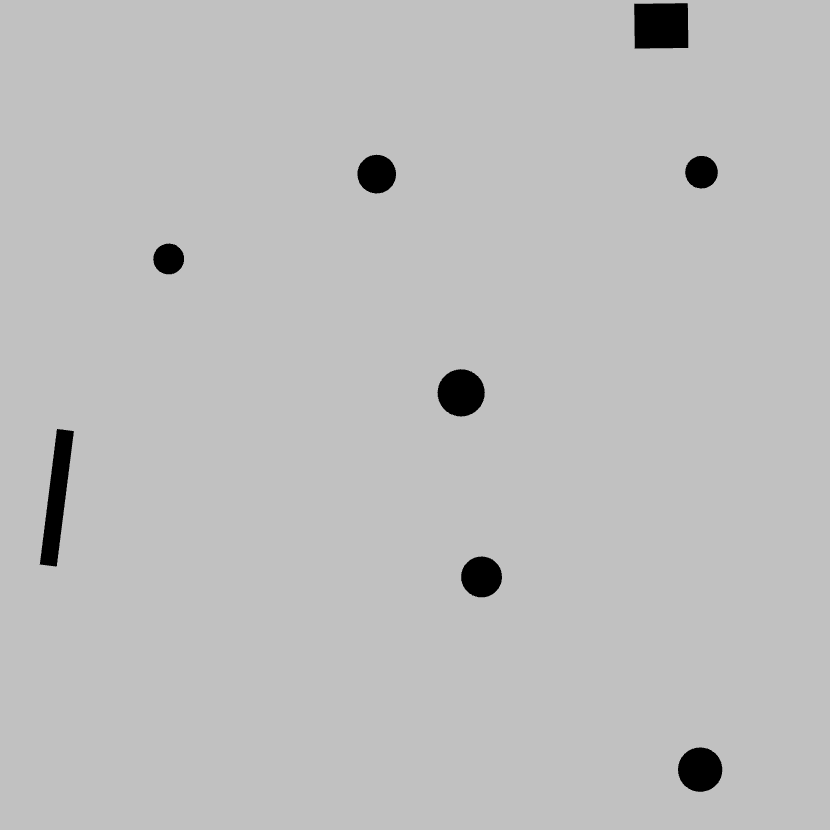
\includegraphics[width=0.15\linewidth]{graphics/test_model_08_2.png}
				\hfill
				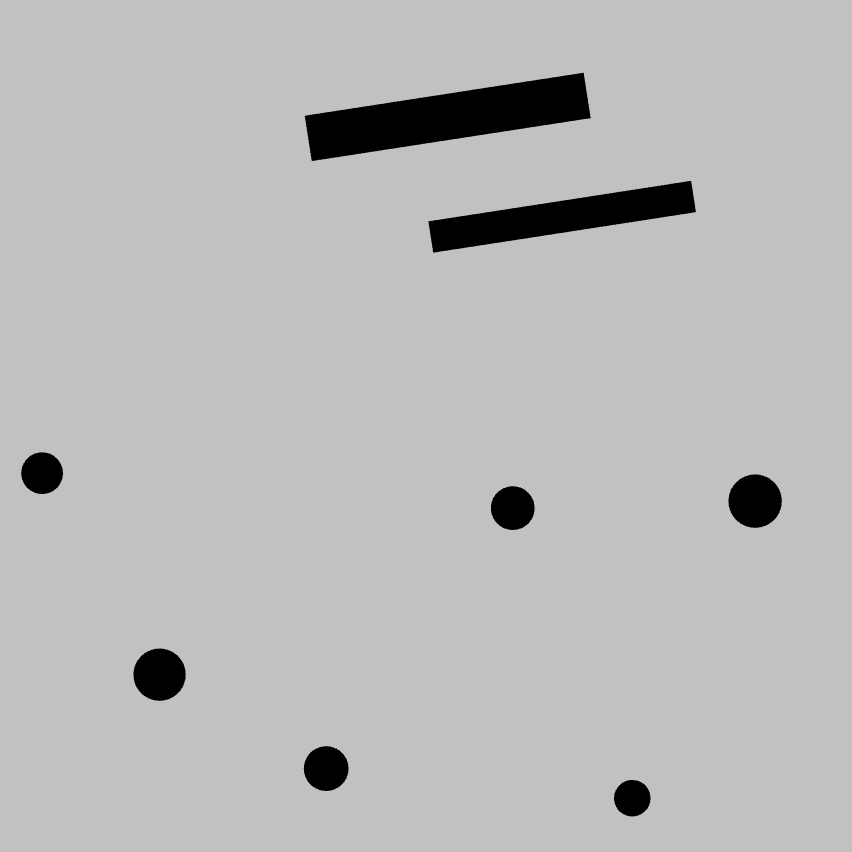
\includegraphics[width=0.15\linewidth]{graphics/test_model_08_3.png}
				\hfill
				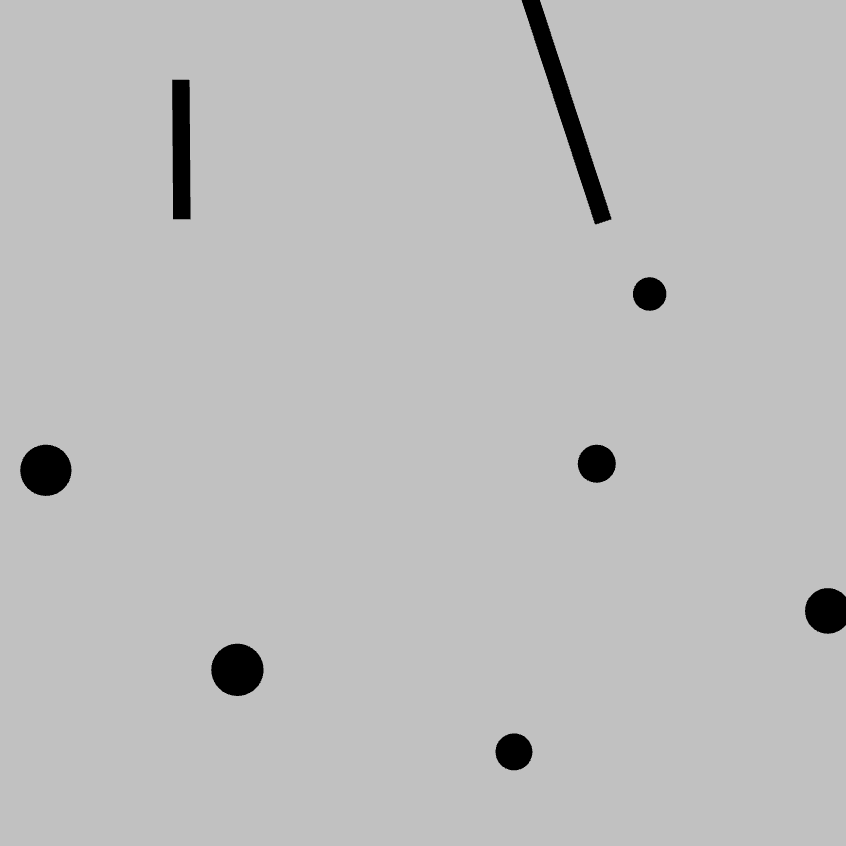
\includegraphics[width=0.15\linewidth]{graphics/test_model_08_4.png}
				\hfill
				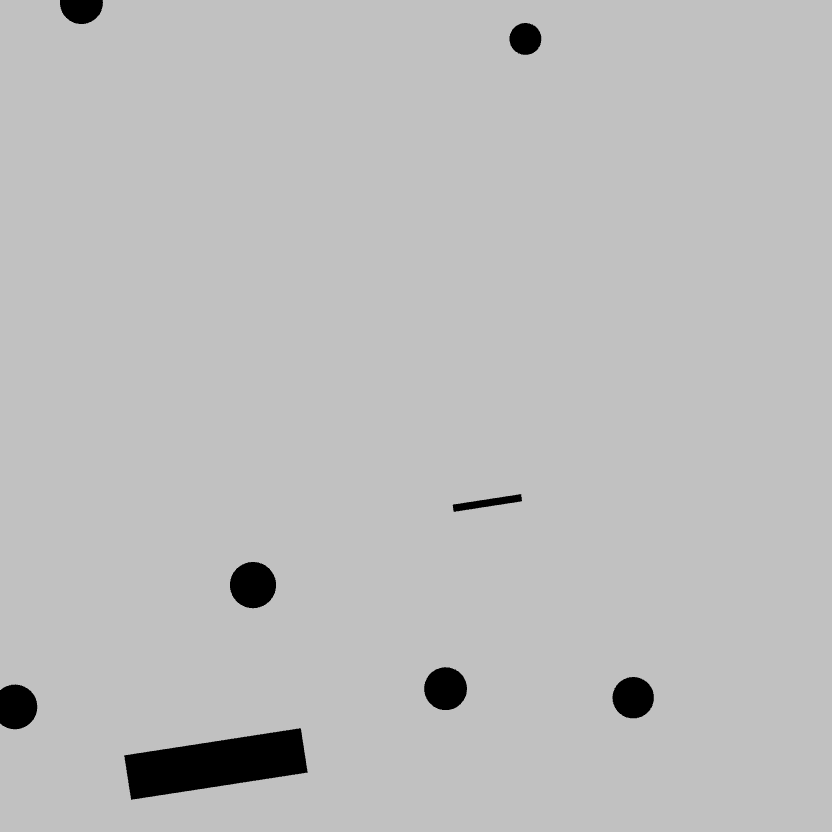
\includegraphics[width=0.15\linewidth]{graphics/test_model_08_5.png}
				\caption{Testing worlds with 8 corrosion areas}
				\label{fig:test_model_08_5}
			\end{subfigure}
			\hfill
			\begin{subfigure}[t]{\linewidth}
				\centering
				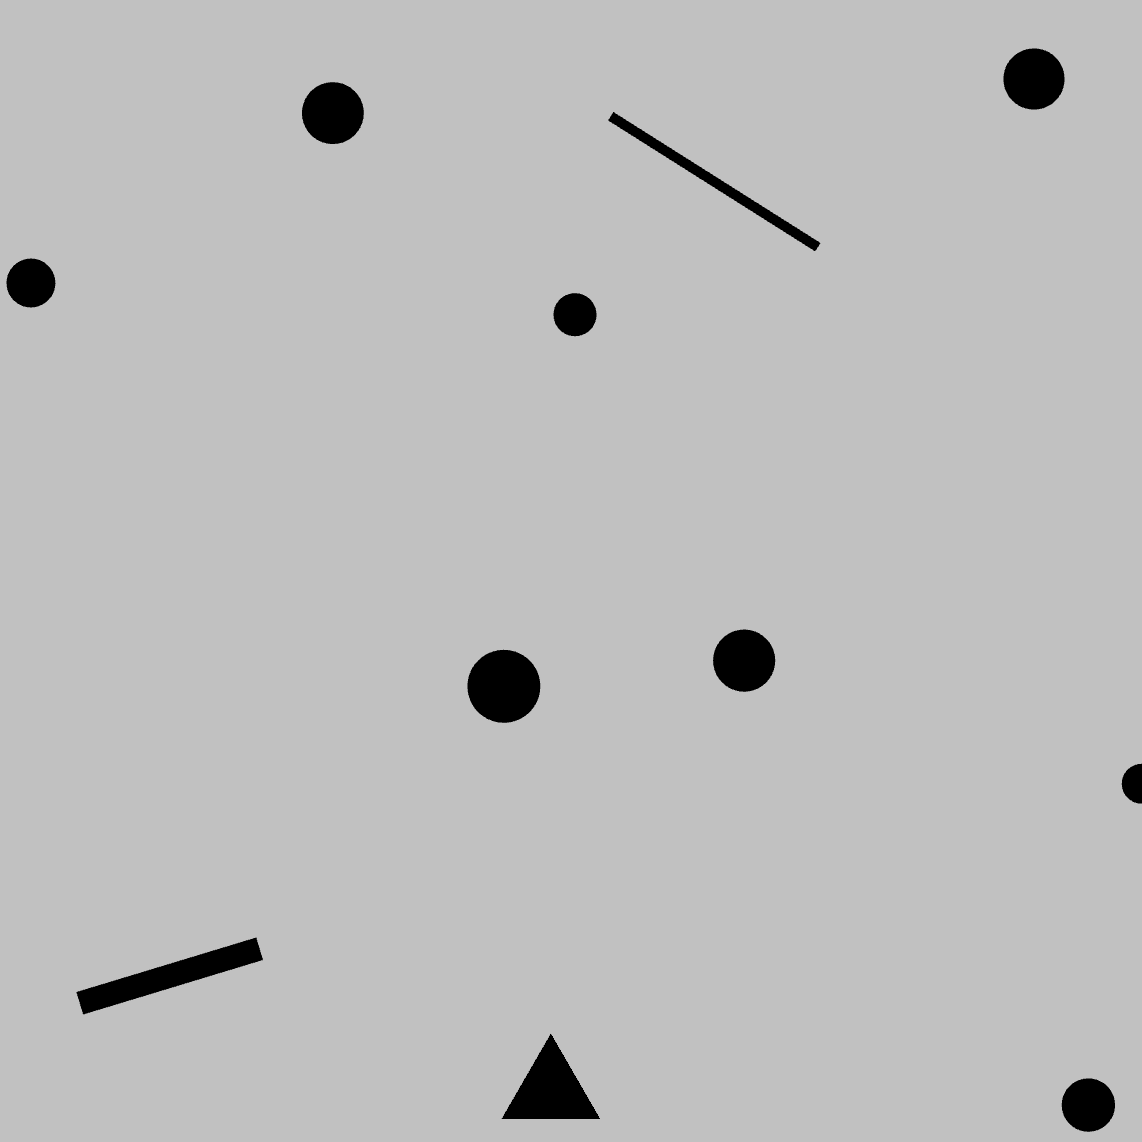
\includegraphics[width=0.15\linewidth]{graphics/test_model_11_1.png}
				\hfill
				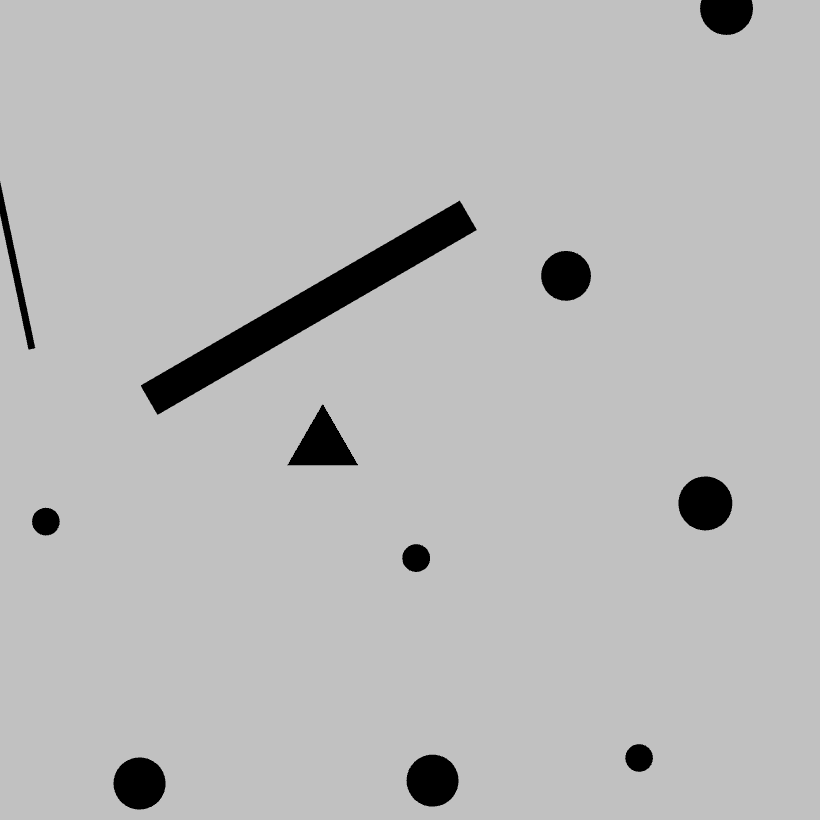
\includegraphics[width=0.15\linewidth]{graphics/test_model_11_2.png}
				\hfill
				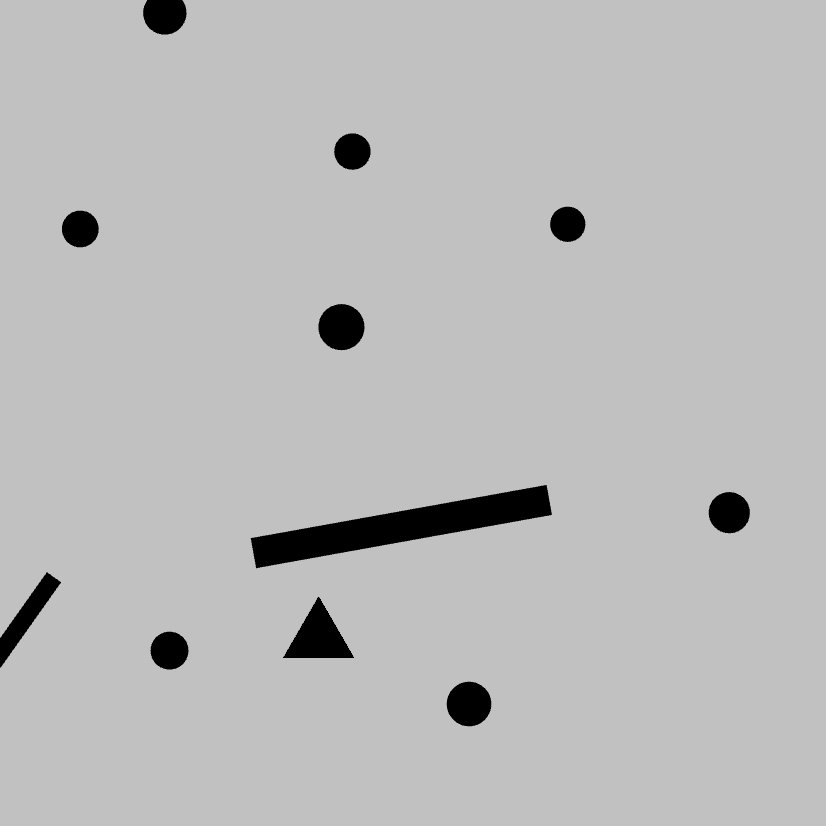
\includegraphics[width=0.15\linewidth]{graphics/test_model_11_3.png}
				\hfill
				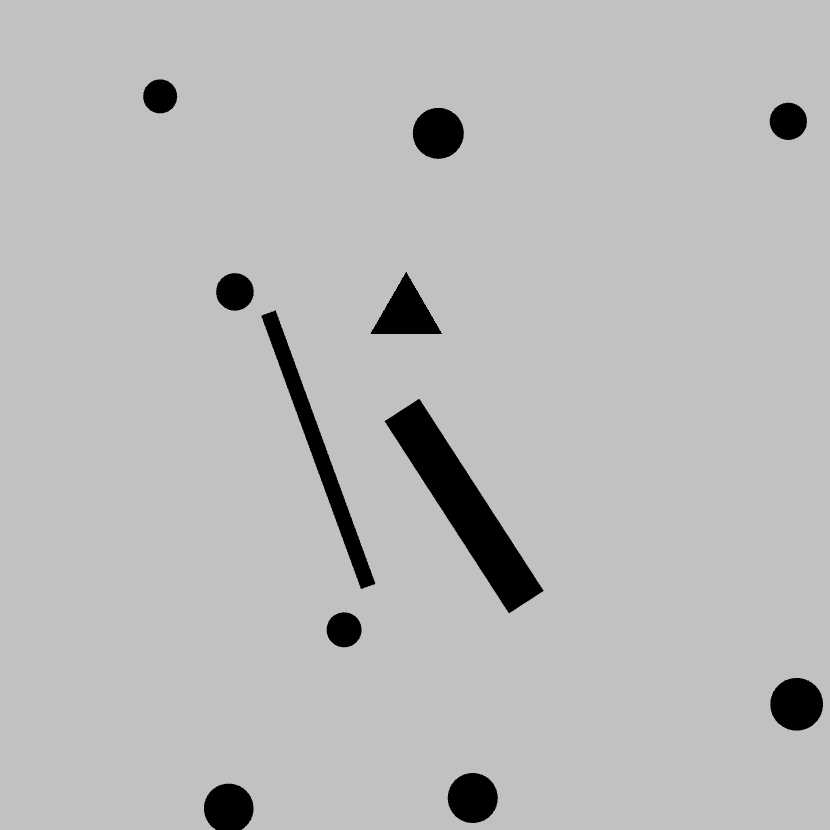
\includegraphics[width=0.15\linewidth]{graphics/test_model_11_4.png}
				\hfill
				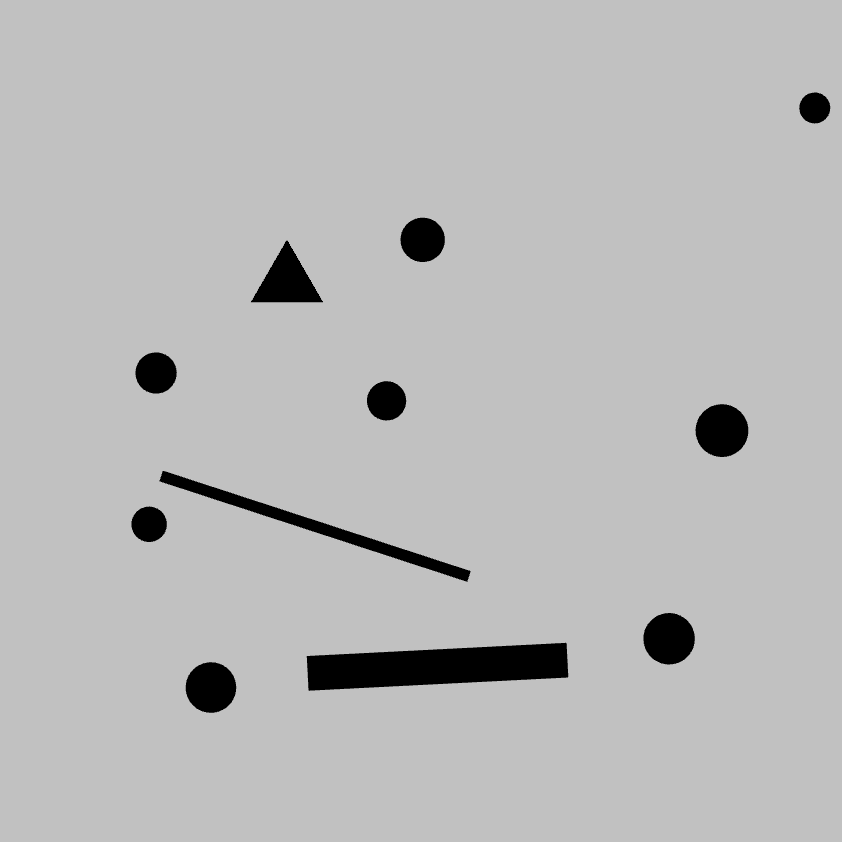
\includegraphics[width=0.15\linewidth]{graphics/test_model_11_5.png}
				\caption{Testing worlds with 11 corrosion areas}
				\label{fig:test_model_11_5}
			\end{subfigure}
			\hfill
			\begin{subfigure}[t]{\linewidth}
				\centering
				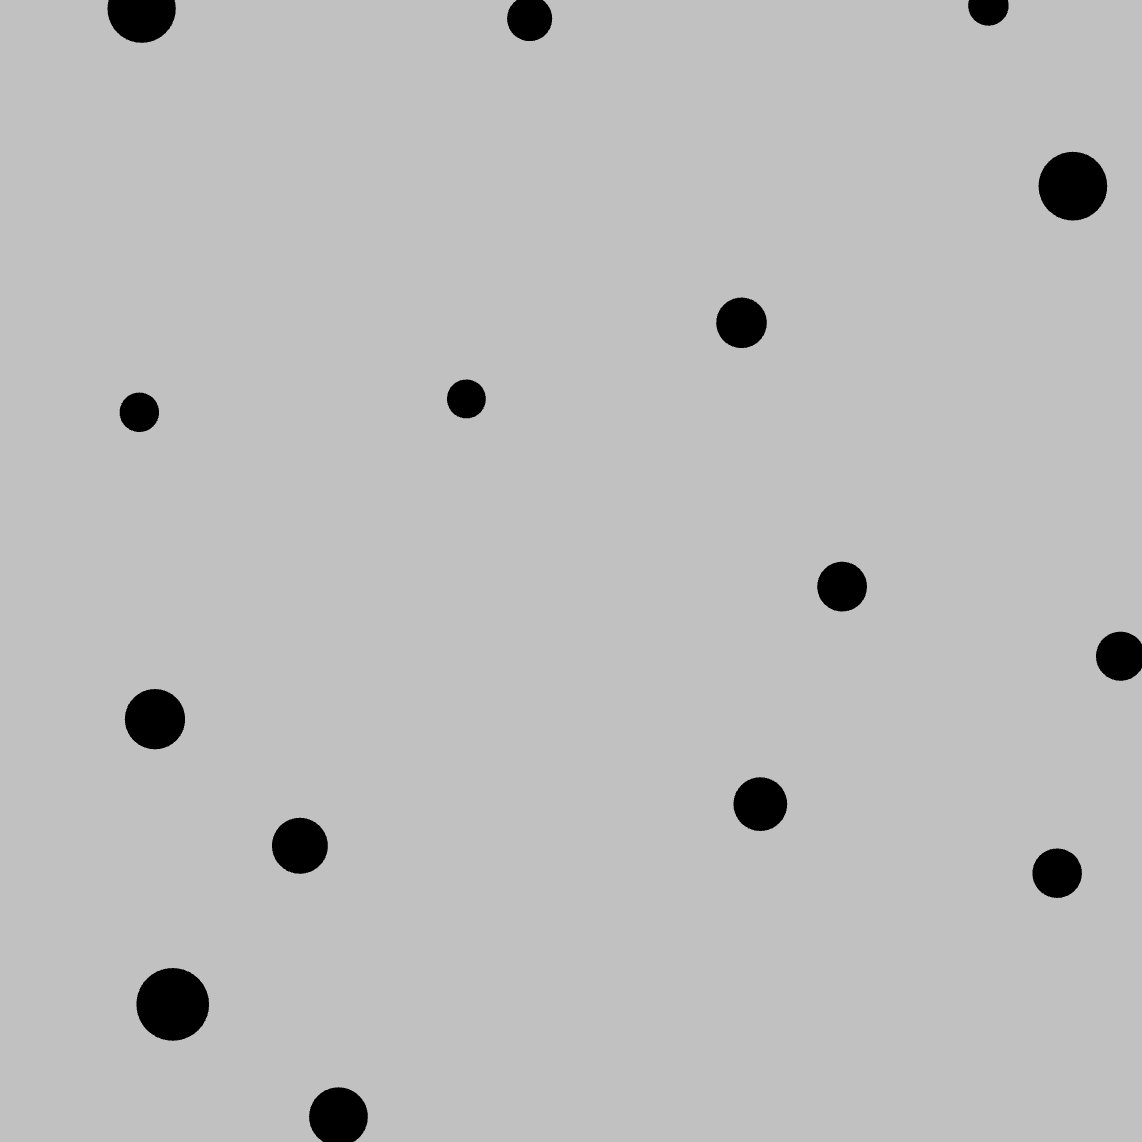
\includegraphics[width=0.15\linewidth]{graphics/test_model_15_1.png}
				\hfill
				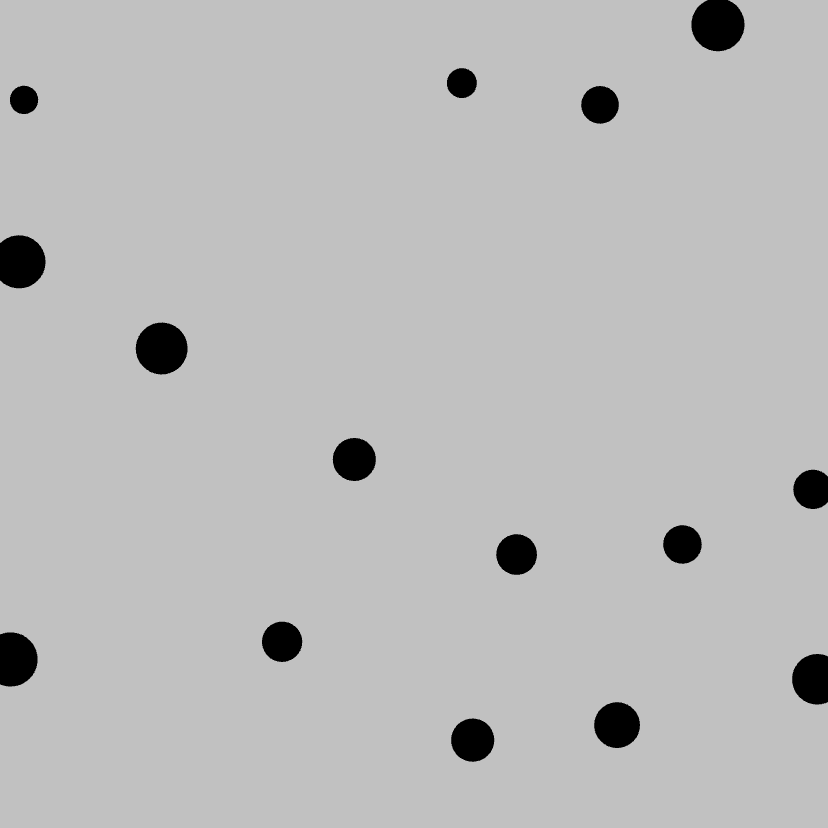
\includegraphics[width=0.15\linewidth]{graphics/test_model_15_2.png}
				\hfill
				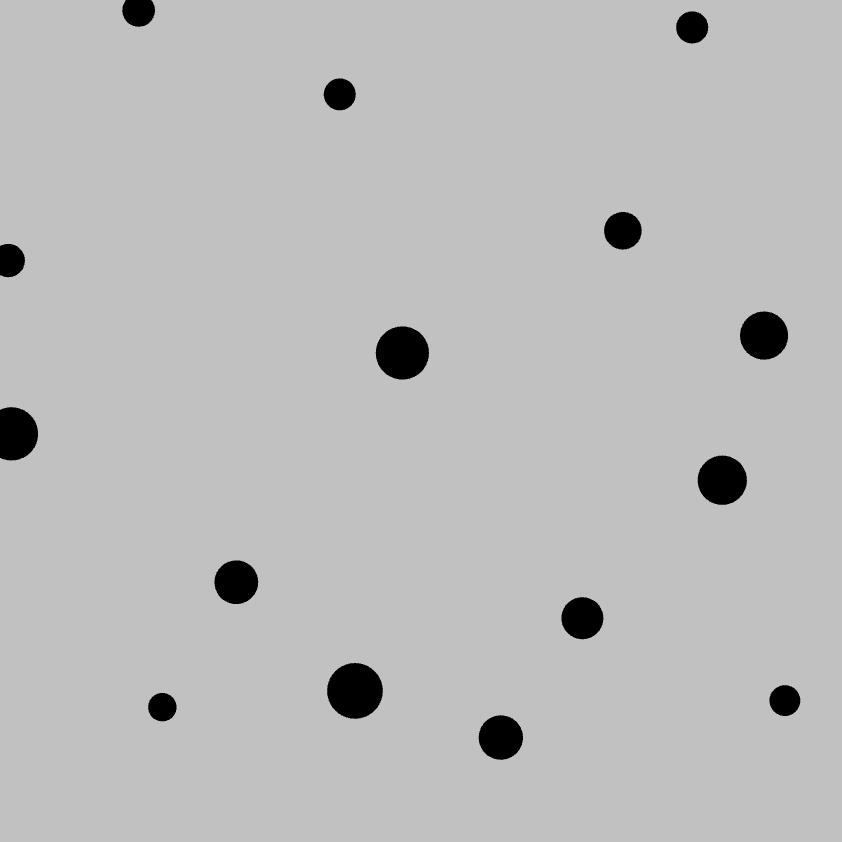
\includegraphics[width=0.15\linewidth]{graphics/test_model_15_3.png}
				\hfill
				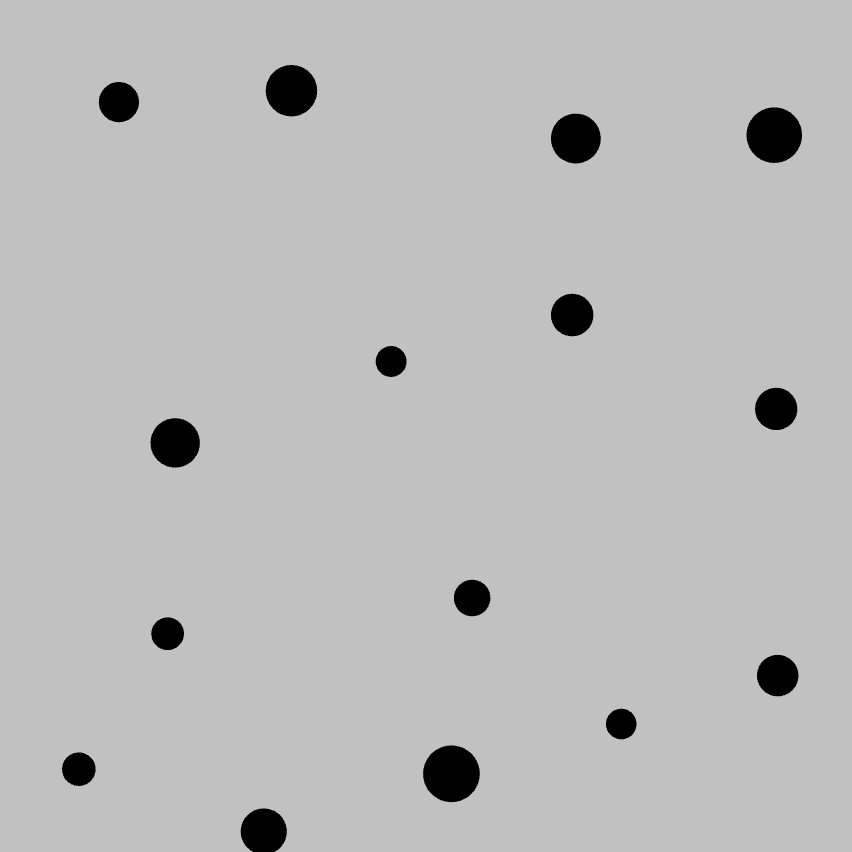
\includegraphics[width=0.15\linewidth]{graphics/test_model_15_4.png}
				\hfill
				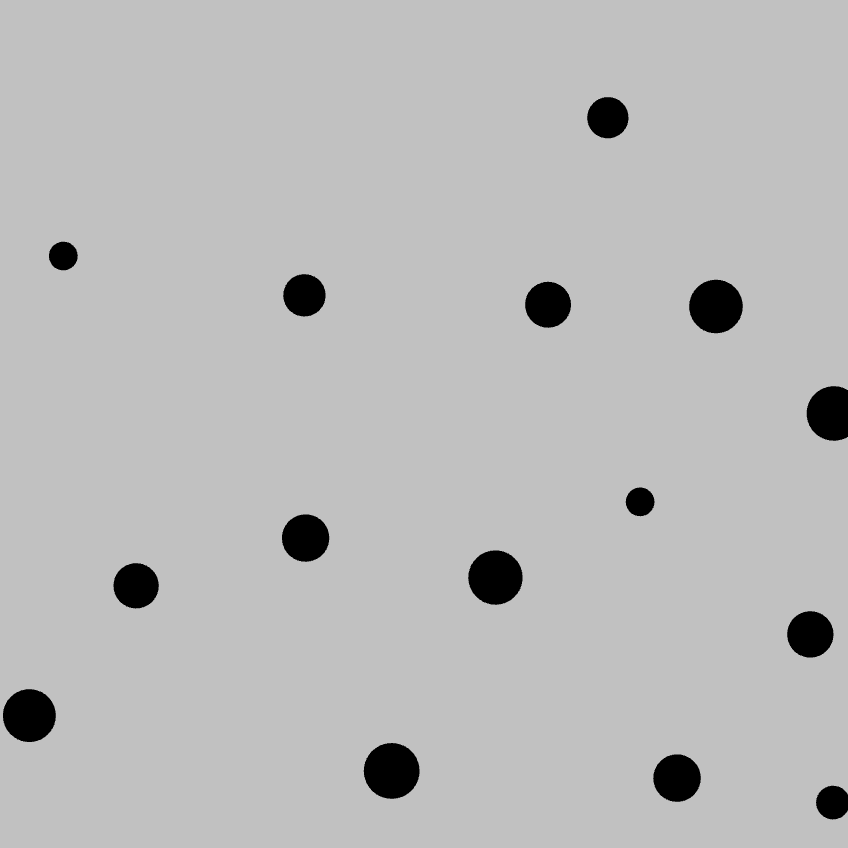
\includegraphics[width=0.15\linewidth]{graphics/test_model_15_5.png}
				\caption{Testing worlds with 15 corrosion areas}
				\label{fig:test_model_15_5}
			\end{subfigure}
			\hfill
			\begin{subfigure}[t]{0.15\linewidth}
				\centering
				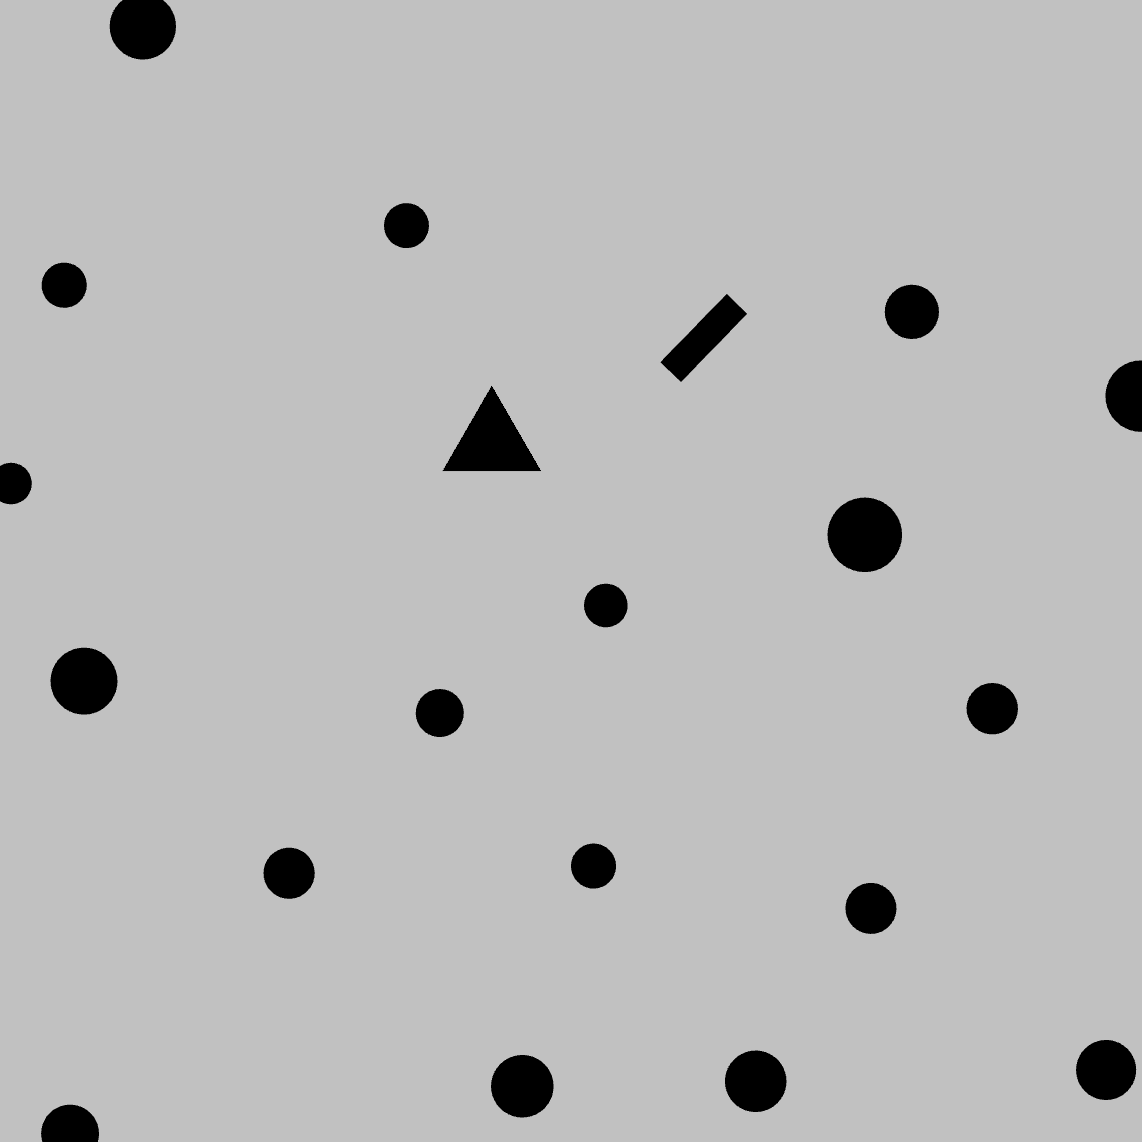
\includegraphics[width=\linewidth]{graphics/test_model_20_1.png}
				\caption{Testing world with 20 corrosion areas}
				\label{fig:test_model_20_1}
			\end{subfigure}
			\hfill
			\begin{subfigure}[t]{0.15\linewidth}
				\centering
				
\includegraphics[width=\linewidth]{graphics/test_model_30_1.png}
				\caption{Testing world with 30 corrosion areas}
				\label{fig:test_model_30_1}
			\end{subfigure}
			\hfill
			\begin{subfigure}[t]{0.15\linewidth}
					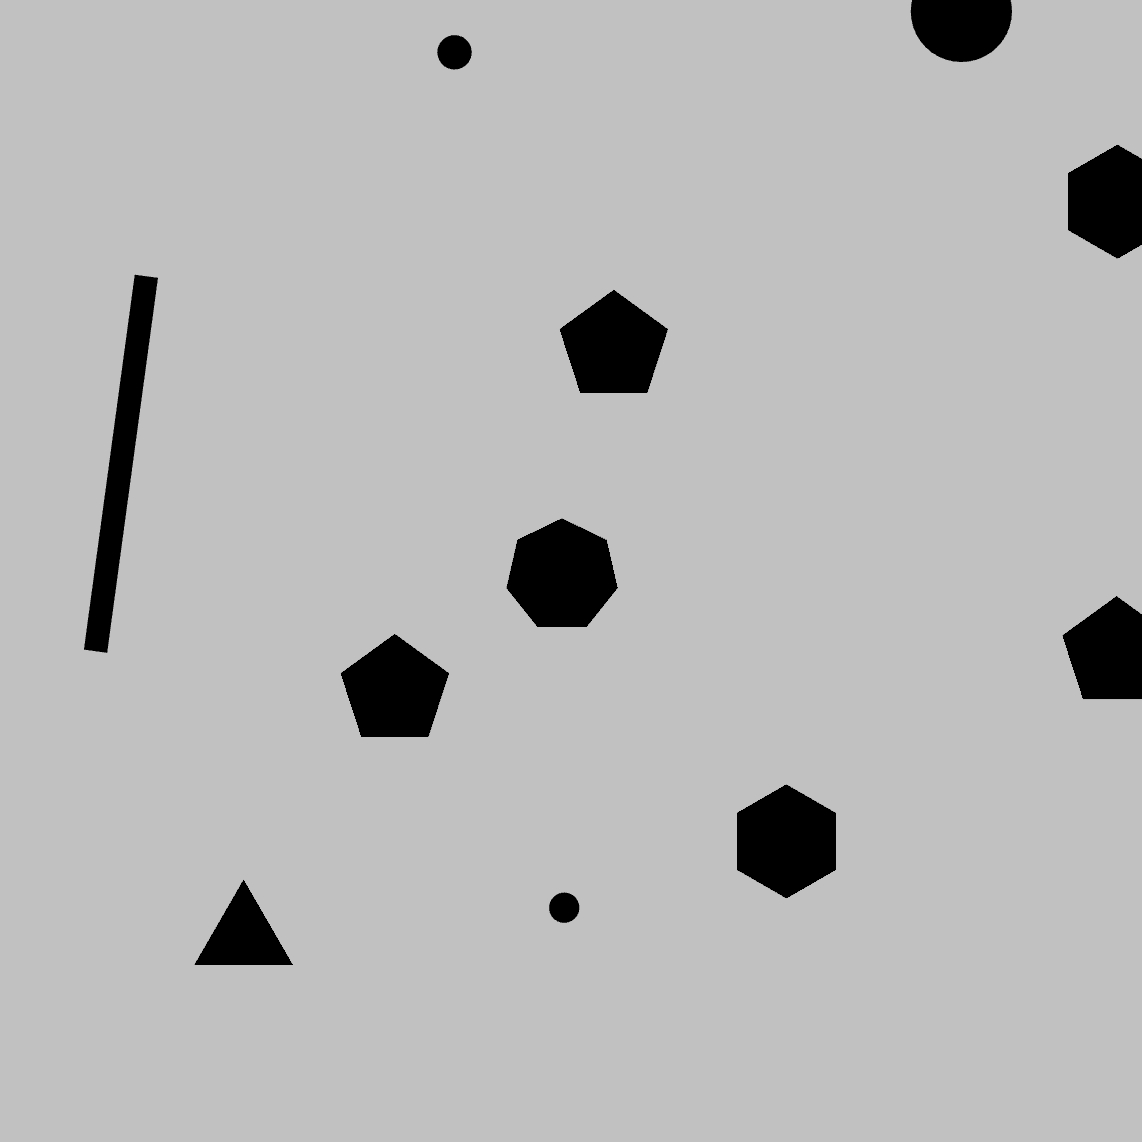
\includegraphics[width=\linewidth]{graphics/test_model_11_complex_1.png}
					\caption{Testing world with 11 complex corrosion areas}
					\label{fig:test_model_11_complex_1}
			\end{subfigure}
			\hfill
			\begin{subfigure}[t]{0.15\linewidth}
				\centering
				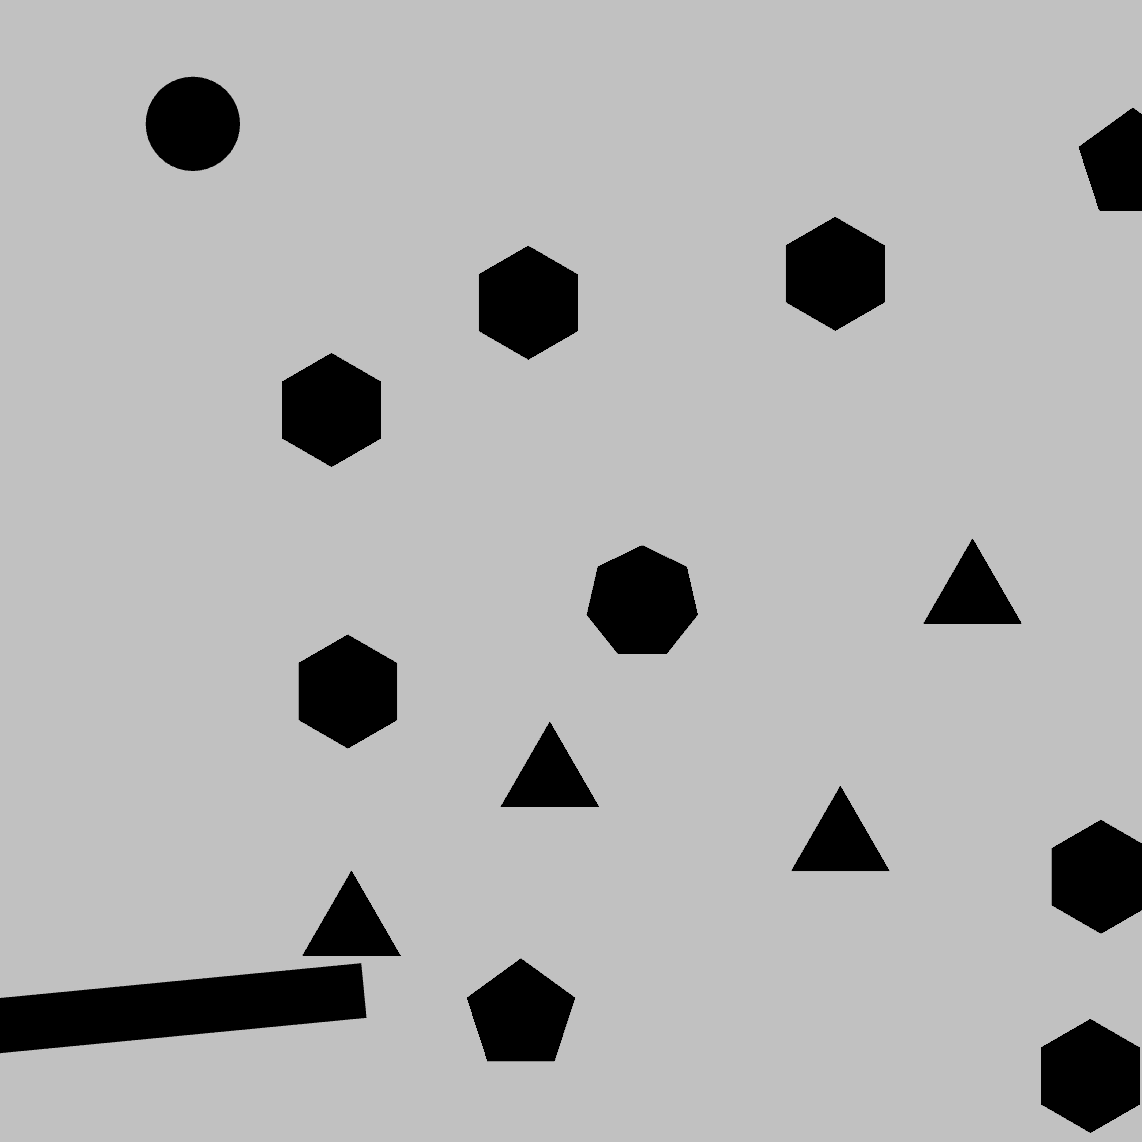
\includegraphics[width=\linewidth]{graphics/test_model_15_complex_1.png}
				\caption{Testing world with 15 complex corrosion areas}
				\label{fig:test_model_15_complex_1}
			\end{subfigure}
			\caption{Différents environnements de test.}
			\label{fig:test_models}
		\end{figure}
	\section{Résultat d'investigation}
		\label{annexe:resultat}
		\TODO{figure avec la superposition des images}
\end{document}

% \begin{Definition}[Proposition (mathématiques)
% 	\footnote{\url{https://www.techno-science.net/definition/6406.html}, dernière visite le 31/10/2019.}]
% 	\label{def:troll}
% 	En mathématiques, dans une théorie donnée, une \textbf{proposition} est un énoncé formé d'un assemblage de symboles et de mots, auquel une valeur de vérité vrai ou faux peut être attribuée, dans certaines conditions mais de la vérité duquel on pourra toujours décider dans toute situation.
% \end{Definition}

% Exemple de proposition~:
% \begin{Proposition}[La Terre sphérique des Anciens\footnote{\url{https://planet-terre.ens-lyon.fr/article/histoire-forme-Terre.xml}, dernière visite le 31/10/2019}]
% 	\label{prop:f}
% 	La Terre est supposée plate, de la forme d'un disque, entièrement ceinturée par le fleuve Océan et recouverte d'un ciel en coupole hémi-sphérique.
% \end{Proposition}

% Pour effectuer une définition
% \begin{Definition}[Troll (internet)
% 	\footnote{\url{https://www.commentcamarche.net/faq/3610-qu-est-ce-qu-un-troll-informatique}, dernière visite le 31/10/2019.}]
% 	\label{def:troll}
% 	Le terme \textbf{troll} désigne, dans le jargon de l'internet, un personnage malfaisant dont le but premier est de perturber le fonctionnement des forums de discussion en multipliant les messages sans intérêt (ou, plus subtilement, en provoquant leur multiplication).
% \end{Definition}

% Lorsque l'on veut écrire des équations
% \begin{equation}
% 	\label{eq:f}
% 	f(x) = 0 \iff x = 1
% \end{equation}

% La définition~\ref{def:troll} n'a aucun lien avec l'équation~\ref{eq:f}.

% \begin{Theorem}[Théorème de Pythagore]
% 	\label{Th:Pythagore}
% 	On nomme $a$, $b$ et $c$ les longueurs des trois côtés d'un triangle.\\
% 	Les triangles pour lesquels on a la relation $a^{2}+ b^{2} = c^{2}$ sont tous les triangles rectangles dont l'hypoténuse est le côté de longueur $c$, et seulement eux.

% 	Source : \url{http://mathematiques3.free.fr/2troisieme/problemes/prob014.php}, dernière visite 31/10/2019.
% \end{Theorem}

% On peut aussi écrire des corolaires
% \begin{Corollary}[]
% 	\label{Cor:TriangleImpossible}
% 	Il n'existe aucun triangle rectangle ayant les longueurs de côté suivantes~: $3$, $2$ et $23$.
% \end{Corollary}

% Reste à le prouver.
% \begin{proof}
% 	Pour prouver ce corollaire, procédons par l'absurde en supposant que le triangle soit rectangle. Il y a alors trois possibilités pour la longueur de l'hypoténuse $c$.
% 	\begin{itemize}
% 		\item $c=3$\\
% 		or $2^{2}+ 23^{2} \neq 3^{2}$\\
% 		donc si le triangle est rectangle, sa longueur ne peut être $3$.
% 		\item $c=2$\\
% 		or $3^{2}+ 23^{2} \neq 2^{2}$\\
% 		donc si le triangle est rectangle, sa longueur ne peut être $2$.
% 		\item $c=23$\\
% 		or $2^{2}+ 3^{2} \neq 23^{2}$\\
% 		donc si le triangle est rectangle, sa longueur ne peut être $23$.
% 	\end{itemize}
% 	Donc aucun côté ne satisfait la définition d'une hypoténuse. Le triangle ne peut donc pas être un triangle rectangle.
% \end{proof}
% Il est aussi possible d'écrire des lemmes.

% \begin{Lemma}[Lemme d'Euclide\footnote{\url{https://fr.wikipedia.org/wiki/Lemme_d'Euclide}, dernière visite le 30/10/2019}]
% 	\label{lem:Euclide}
% 	Si un nombre premier $p$ divise le produit de deux nombres entiers $b$ et $c$, alors $p$ divise $b$ ou $c$.
% \end{Lemma}